\documentclass[journal,twoside,web]{ieeecolor}
\usepackage{generic}
\usepackage{cite}
\usepackage{amsmath,amssymb,amsfonts}
\usepackage{algorithmic}
\usepackage{algorithm,algorithmic}
\usepackage{hyperref}
\hypersetup{hidelinks=true}
\usepackage{textcomp}
\usepackage{tabularx} % 引入tabularx包
\usepackage{subcaption}

\def\BibTeX{{\rm B\kern-.05em{\sc i\kern-.025em b}\kern-.08em
    T\kern-.1667em\lower.7ex\hbox{E}\kern-.125emX}}
\markboth{\hskip25pc MATLAB Language and Simulation Lab}
{Xiaotao Li \MakeLowercase{\textit{et al.}}: Real-time Simulation PID Controller Design}
\begin{document}
\title{Real-time Simulation PID Controller Design}
% \author{First A. Author, \IEEEmembership{Fellow, IEEE}, Second B. Author, and Third C. Author Jr., \IEEEmembership{Member, IEEE}
\author{Xiaotao Li, Yikai Kang
% \thanks{This paragraph of the first footnote will contain the date on 
% which you submitted your paper for review. It will also contain support 
% information, including sponsor and financial support acknowledgment. For 
% example, ``This work was supported in part by the U.S. Department of 
% Commerce under Grant 123456.'' }
% \thanks{The next few paragraphs should contain 
% the authors' current affiliations, including current address and e-mail. For 
% example, First A. Author is with the National Institute of Standards and 
% Technology, Boulder, CO 80305 USA (e-mail: author@boulder.nist.gov). }
% \thanks{Second B. Author Jr. was with Rice University, Houston, TX 77005 USA. He is 
% now with the Department of Physics, Colorado State University, Fort Collins, 
% CO 80523 USA (e-mail: author@lamar.colostate.edu).}
\thanks{Xiaotao Li is with the College of Mechatronics and Control Engineering, Shenzhen University, Shenzhen, 518060, China (e-mail: 2310295083@email.szu.edu.cn).}
\thanks{Yikai Kang is with the College of Mechatronics and Control Engineering, Shenzhen University, Shenzhen, 518060, China (e-mail: 2310295084@email.szu.edu.cn).}}


\maketitle

\begin{abstract}
This paper presents the design and implementation of a PID (Proportional-Integral-Derivative) controller enhanced with real-time simulation capabilities, developed using MATLAB and APP Designer. Central to the study is the application of this controller to the inverted pendulum on a cart, a benchmark challenge in control theory. The controller integrates advanced PID tuning mechanisms within a user-friendly graphical interface, facilitating dynamic parameter adjustments and visualization of system responses in real-time. Key features of the system include customizable input signal configuration, transfer function modification, and PID parameter optimization. Experimental results demonstrate the efficacy of the controller in maintaining the stability of the inverted pendulum system under various operating conditions, showcasing significant improvements in tuning efficiency and system responsiveness.
\end{abstract}

\begin{IEEEkeywords}
PID Controller, Inverted Pendulum, Control System Design, Parameter Tuning
\end{IEEEkeywords}

\section{Introduction}
\label{sec:introduction}
\IEEEPARstart{I}{n} modern industrial control systems, PID (Proportional-Integral-Derivative) controllers are widely used due to their simple structure, convenient adjustment, and robust performance. They effectively manage the output of various dynamic systems to achieve the desired control effects. PID controllers[1] play a crucial role in many fields, such as robotics, the automotive industry, and aerospace. In my research project, I am dedicated to designing an effective controller for the altitude control of a latex balloon (aerostat)[2],[3]. The core technology involves precise control over the exhaust and ballast actuators to adjust the net buoyancy and the weight of the aerostat, ensuring stable operation of the balloon within a predetermined height range. After comparative analyses, the PID controller has become the preferred option for altitude control due to its high efficiency and reliability.

\subsection{Research Motivation}
Although the theory and application of PID controllers are relatively mature, rapidly and effectively tuning PID parameters according to specific system characteristics remains a significant challenge in practice. Additionally, the lack of intuitive visualization tools makes it difficult to monitor and assess control effects in real-time. Thus, designing a PID regulator that can visually display control effects is of great importance, as it will help optimize the controller design process and improve tuning efficiency. This project uses the inverted pendulum on a cart[4] as a practical application scenario, not only because it is a classic problem in control theory but also because it can effectively demonstrate and test the simulation effects of PID control strategies. Through dynamic modeling, the system transfer function model of the inverted pendulum on a cart was obtained and imported into the workspace, enabling dynamic response curves and animation visualization, making the PID parameter adjustment process more intuitive and comprehensible.

\subsection{Objectives and Structure}
The main objective of this report is to provide a detailed introduction to the design and implementation of a PID regulator developed through MATLAB[5] and APP Designer. This includes the definition of input signals, the establishment of the system model, the methods for PID parameter adjustment, and the implementation of visual responses and animations. The structure of the report will cover the theoretical foundation, system design and implementation, functional realization and experimental results, and conclusions and outlook, offering a comprehensive demonstration of the PID controller design and experimental process, providing the reader with a deep understanding and practical examples of application.


\section{Theoretical Foundation}

\subsection{PID Control Theory and Block Diagram}
The PID controller is the most commonly used feedback controller in industrial control systems, operating on the principle of error computation, which is the difference between the set point and the actual output[6]. The block diagram of the PID controller is shown in Fig.\ref{PID} and consists of three main parts:
\begin{figure}[!t]
\centerline{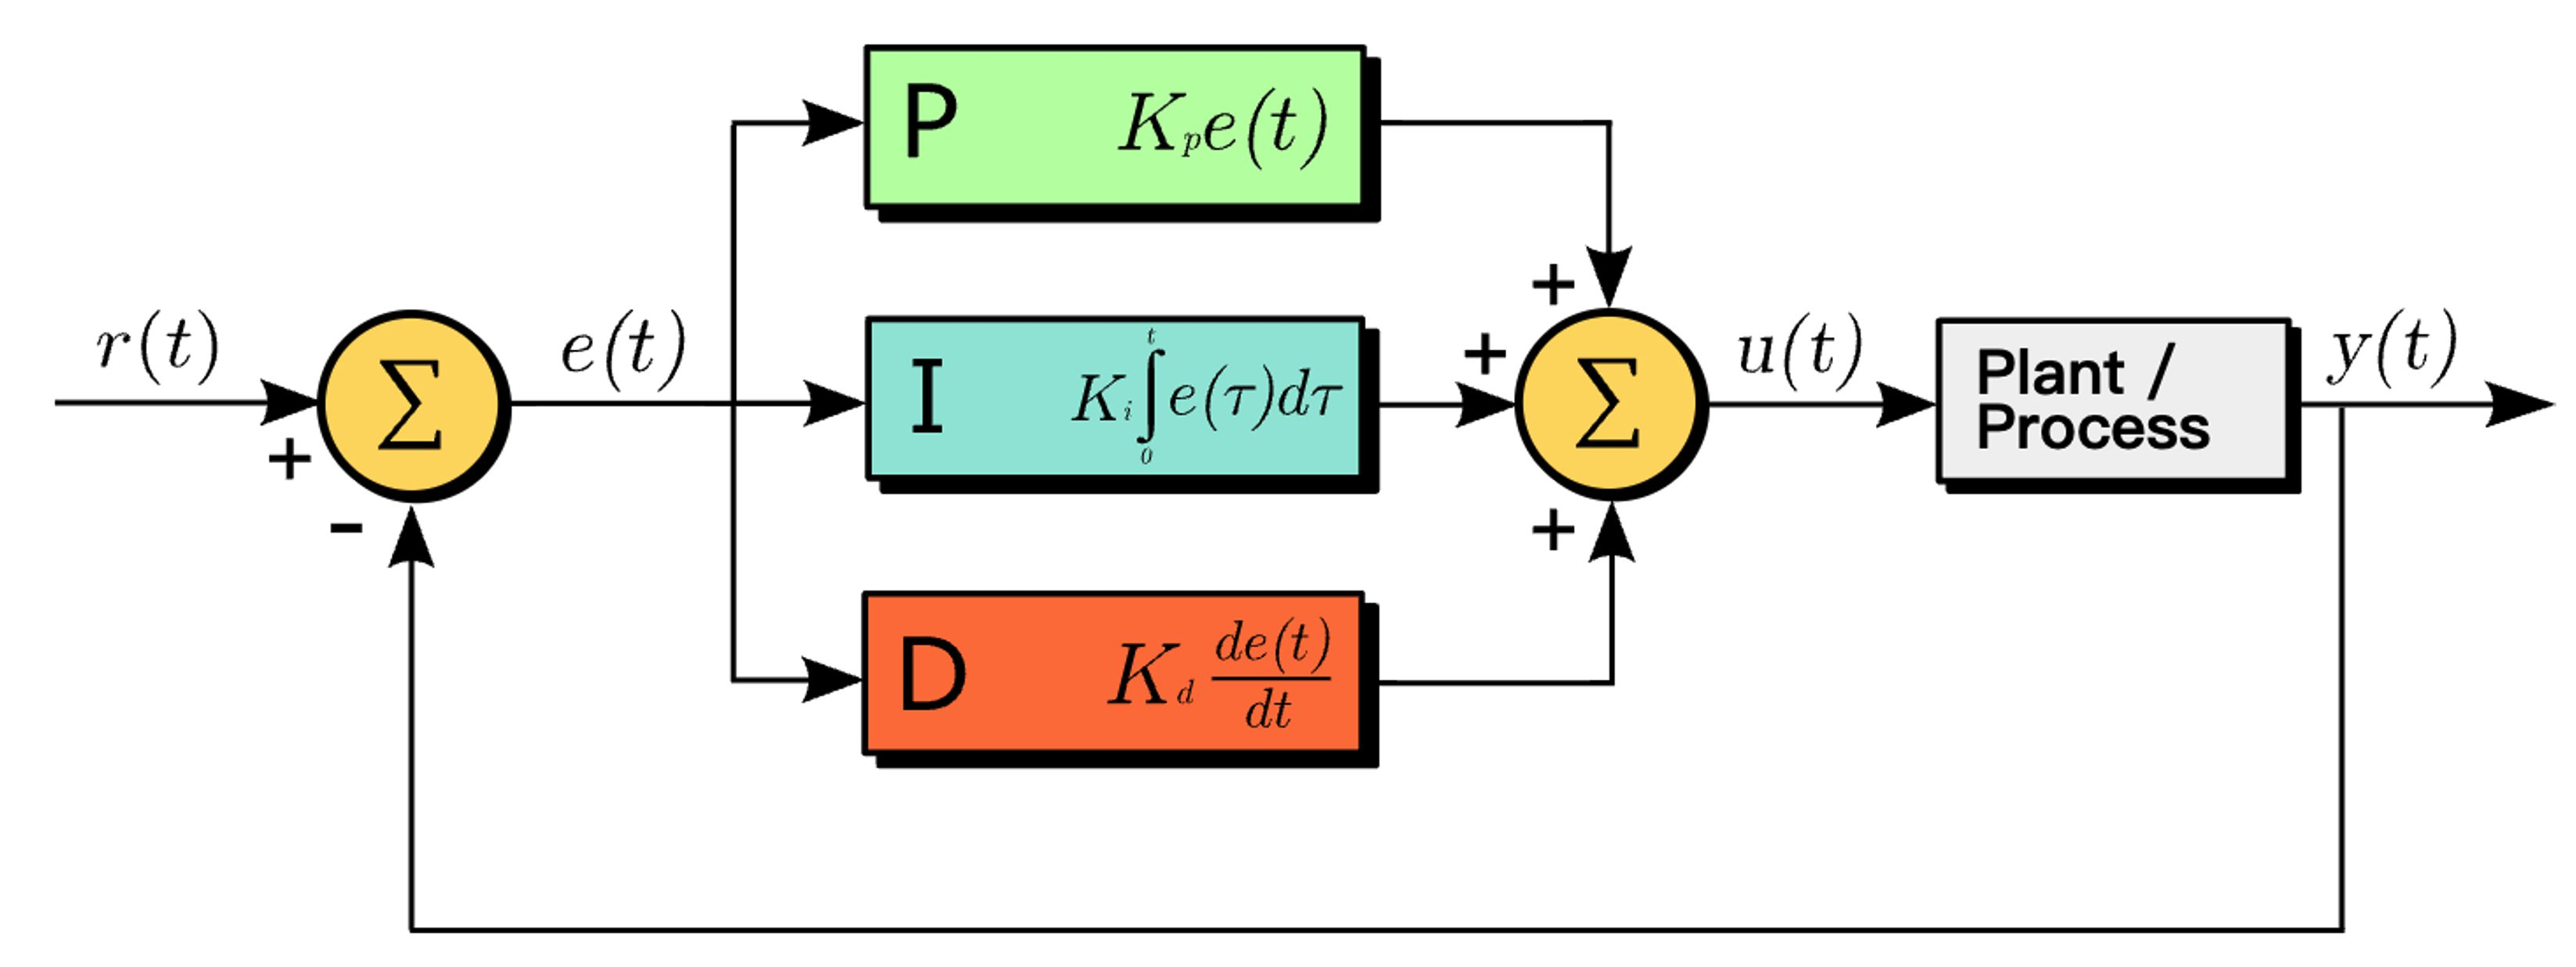
\includegraphics[width=\columnwidth]{Images/PID.jpg}}
\caption{The block diagram of the PID controller}
\label{PID}
\end{figure}

\subsubsection{Proportional Control (P)}
{Proportional control generates a control action that is proportional to the error magnitude, reducing the error. A higher proportional gain \( K_p \) increases system response speed but may lead to overshooting and oscillations if too high.}

\subsubsection{Integral Control (I)}
{Integral control aims to eliminate steady-state error by integrating the error over time. As the error persists, the integral term increases until the error reaches zero. The integral gain \( K_i \) governs the speed and effectiveness of this integration.}

\subsubsection{Derivative Control (D)}
{Derivative control predicts future errors by controlling the rate of change of the error, which helps quickly mitigate the growth of future errors and reduce overshooting. The derivative gain \( K_d \) controls the sensitivity to rapid changes in the error.}


In the diagram, \( e(t) \) represents the error signal, which is the difference between the set point and the measured value, and \( u(t) \) is the controller output. This block diagram illustrates how the controller output is calculated based on the error, incorporating the additive effects of proportional, integral, and derivative calculations.


\subsection{Input Signals and System Modeling}
Classic input signals are plotted in Fig.\ref{input} and include:

\begin{figure}[!t]
\centerline{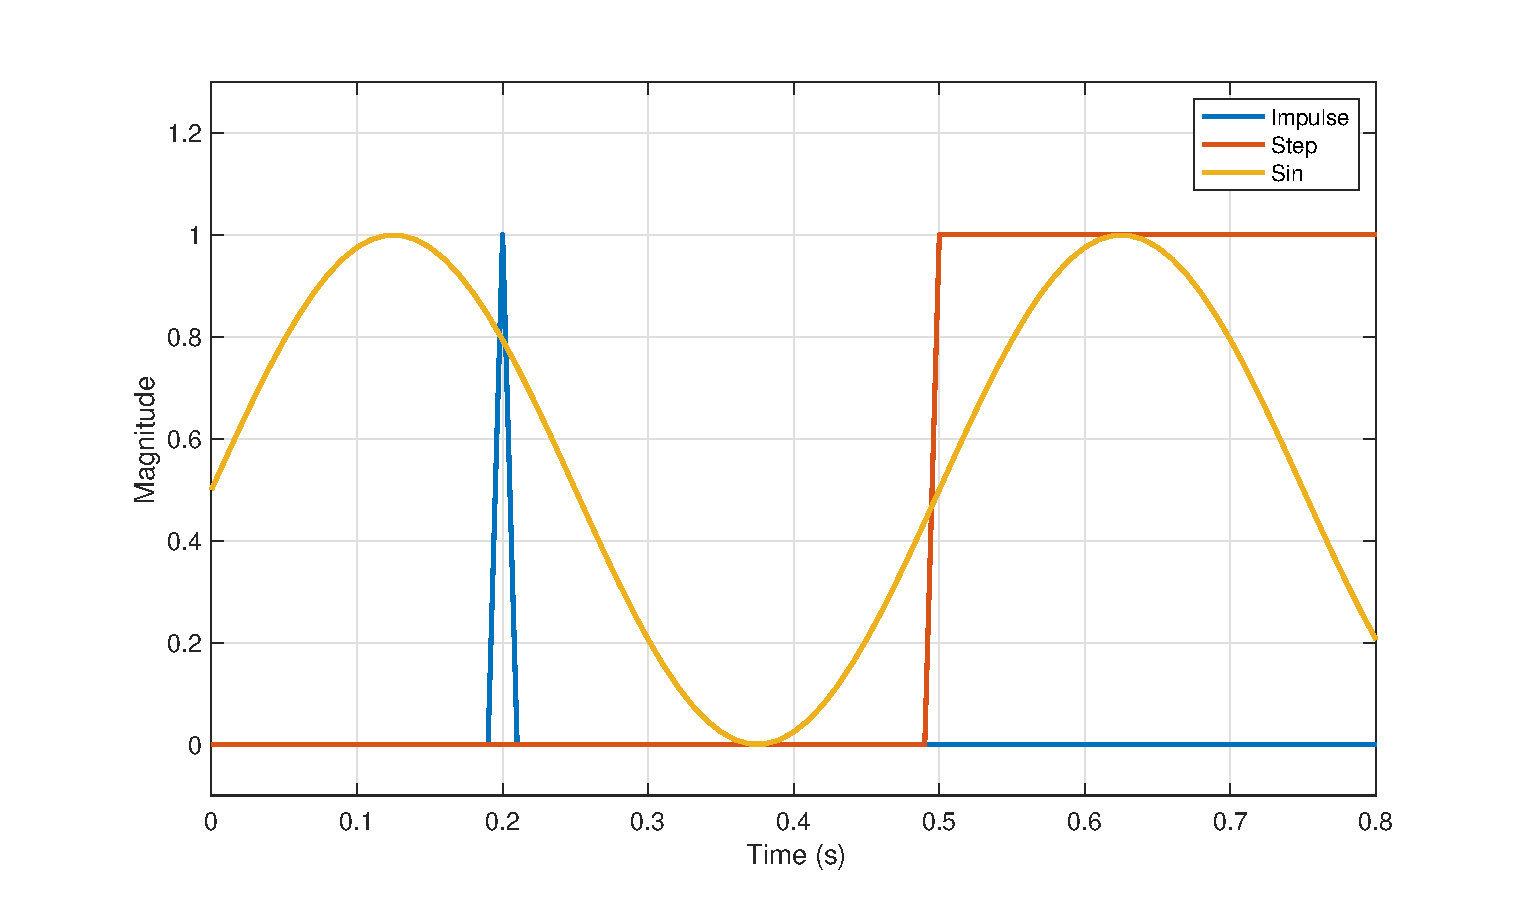
\includegraphics[width=\columnwidth]{Images/input.eps}}
\caption{Comparison of classic input signals.}
\label{input}
\end{figure}

\subsubsection{Step Signal}
{An idealized signal where the value suddenly changes from zero to a constant at a specific moment.}

\subsubsection{Impulse Signal}
{A signal of a certain magnitude applied instantaneously, commonly used to test the transient response of a system.}

\subsubsection{Sine Signal}
{A periodically varying signal, is used to test the system's response to periodic external disturbances.}


\subsection{Modeling of the Inverted Pendulum System on a Cart}

\begin{figure}[!t]
\centerline{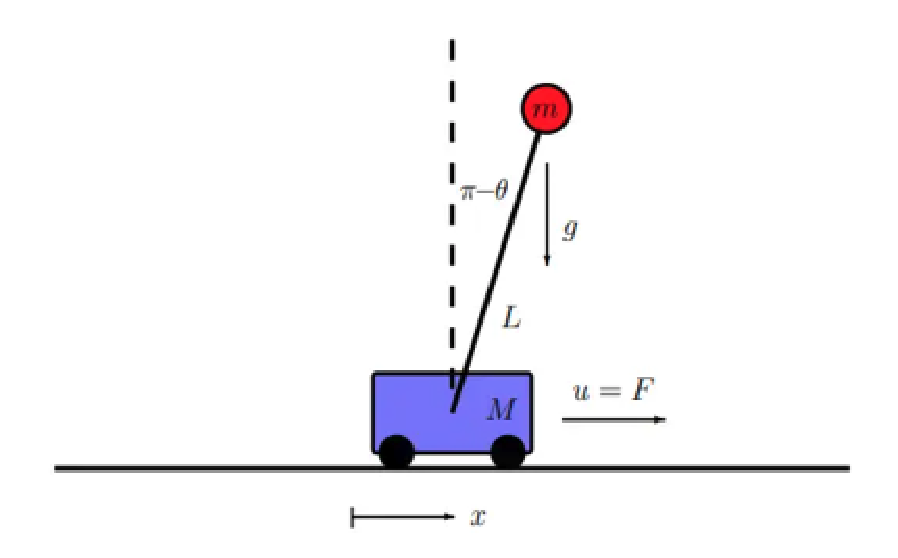
\includegraphics[width=\columnwidth]{Images/Pendulum.eps}}
\caption{Schematic diagram of an inverted pendulum.}
\label{Pendulum}
\end{figure}

The inverted pendulum system on a cart is a classic example of a nonlinear system, widely used in control system education and research[7]. The modeling typically begins with Newtonian mechanics, by deriving the force balance equations for both the pendulum and the cart. These equations are then simplified into a linear state-space model or a transfer function, which is used for designing the PID controller. 

Fig.\ref{Pendulum} is a schematic diagram of the classic inverted pendulum system on a cart. And the physical parameters are included in TABLE\ref{tab:parameters}. The input to the system is the force \(u = F\) applied to the cart. The observable state variables include the cart's position coordinate \(x\) and the pendulum's angle \(\theta\).

\begin{table}[htb]
\caption{Physical Parameters for Inverted Pendulum}
\label{tab:parameters}
\setlength{\tabcolsep}{3pt}  % 调整列间距
\begin{tabular}{|c|c|c|}  % 列格式保持居中
\hline
Symbol & Parameters & Value \\
\hline
\hspace{5mm}$g$\hspace{5mm} & \(-10\) m/s\(^2\) & Gravity  \\
\hspace{5mm}$M$\hspace{5mm} & 5 kg & Cart Mass  \\  % 在单元格内容前后添加空白
\hspace{5mm}$m$\hspace{5mm} & 1 kg & Pendulum Mass  \\
\hspace{5mm}$L$\hspace{5mm} & 2 m & Pendulum Length  \\

\hspace{5mm}$d$\hspace{5mm} & 1 N/m/sec & Damping Coefficient  \\
\hspace{5mm}$s$\hspace{5mm} & 1 & Pendulum Initial State  \\
\hline
\multicolumn{3}{p{240pt}}{Note: $m$ = meter, $s$ = second, $kg$ = kilogram.}  
\end{tabular}
\end{table}

Summing the forces in the free-body diagram of the cart in the horizontal direction,  get the following equation of motion:
\begin{equation}M\ddot{x}+b\dot{x}+N=F\label{eq1}\end{equation}

Summing the forces in the free-body diagram of the pendulum in the horizontal direction,  get the following expression for the reaction force $N$:
\begin{equation}N=m\ddot{x}+ml\ddot{\theta}\cos\theta-ml\dot{\theta}^2\sin\theta \label{eq2}\end{equation}

substitute equation \eqref{eq2} into the equation \eqref{eq1}, get one of the two governing equations for this system:
\begin{equation}(M+m)\ddot{x}+b\dot{x}+ml\ddot{\theta}\cos\theta-ml\dot{\theta}^2\sin\theta=F\label{eq3}\end{equation}

Sum the forces perpendicular to the pendulum to get the second equation of motion for this system:
\begin{equation}P\sin\theta+N\cos\theta-mg\sin\theta=ml\ddot{\theta}+m\ddot{x}\cos\theta \label{eq4}\end{equation}

Sum the moments about the centroid of the pendulum to get rid of the $P$ and $N$ terms in the equation \eqref{eq4} to get the following equation:
\begin{equation}-Pl\sin\theta-Nl\cos\theta=I\ddot{\theta}\label{eq5}\end{equation}

Combining equation \eqref{eq4} and equation \eqref{eq5} to get the second governing equation:
\begin{equation}(I+ml^2)\ddot{\theta}+mgl\sin\theta=-ml\ddot{x}\cos\theta \label{eq6}\end{equation}

This set of equations needs to be linearized. So presuming a small deviation ($\phi$) from equilibrium, use the following small angle approximations of the nonlinear functions in  system equations:

\begin{equation}\label{eq7}\begin{aligned}\cos\theta&=\cos(\pi+\phi)\approx-1 ,\\\\\sin\theta&=\sin(\pi+\phi)\approx-\phi,\\\\\dot\theta^2&=\dot\phi^2\approx0\end{aligned}\end{equation}

After subsisting the above approximations into nonlinear governing equations, arrive at the two linearized equations of motion:
\begin{equation}\label{eq8}\begin{aligned}&(I+ml^2)\ddot{\phi}-mgl\phi=ml\ddot{x},\\\\&(M+m)\ddot{x}+b\dot{x}-ml\ddot{\phi}=u\end{aligned}\end{equation}

The system can be described by the cart's position \(x\), velocity \(\dot{x}\) , and the pendulum's angle \(\theta\) ,angular velocity \(\dot{\theta}\).This leads to the equation of state of the system:
\begin{equation}\begin{array}{l}{\dot{x}=Ax+bu}\\{y=Cx+Du}\end{array}\label{eq9}\end{equation}
where
\begin{equation}\label{eq10}A=\begin{bmatrix}0&1&0&0\\0&-\frac{d} M&s\frac{mg}M&0\\0&0&0&1\\0&-s\frac{d}{ML}&-s\frac{(m+M)g}{ML}&0\end{bmatrix},\end{equation}
and
\begin{equation}\label{eq11}B=\begin{bmatrix}0\\\frac{1}{M}\\0\\s\frac{1}{ML}\end{bmatrix},\end{equation}
and
\begin{equation}\label{eq12}C=\begin{bmatrix}0&0&1&0\end{bmatrix},\end{equation}
and
\begin{equation}\label{eq13}D=\begin{bmatrix}0\end{bmatrix}\end{equation}

To facilitate the design of the PID controller, we focus on the angle of the pendulum as the output of interest, aiming to maintain the pendulum in a vertically upright position. This is achieved by controlling the movement of the cart to stabilize the pendulum.
To convert the system's state-space equations into a transfer function and import it into the workspace , we provide the necessary system model for the subsequent visualization of the PID controller.

\section{System Design and Implementation}

\subsection{Overview of Code Implementation}
In this project, the essence of system design and implementation revolves around the effective integration of a PID controller with the inverted pendulum model on a cart, all simulated within the MATLAB environment. Real-time visualization of the PID control tuner is facilitated through an application developed using App Designer. The coding process involves integration of the system model with the PID controller,  the realization of the dynamic model and its visualization for the inverted pendulum. This section primarily discusses the core functionalities, outlining their design logic and code implementation.

% \subsubsection{Generation and Definition of Input Signals}
% In control systems, appropriate input signals form the basis for effective control. Three typical input signals are used: step, impulse, and sine signals, each catering to different control scenarios. Step signals are utilized to test the system's steady-state performance; impulse signals are used to observe the system's transient response; and sine signals are employed to analyze the system’s ability to counter periodic external disturbances.

\subsubsection{Integration of System Model}
The integration of the system model with the PID controller involves setting up the transfer function, configuring zeros and poles, and importing the system model. This part integrates the system model and controller into a closed-loop system via MATLAB scripts, enabling the generation of response graphs under various parameters by setting the PID controller’s proportional gain ($K_p$), integral gain ($K_i$), and derivative gain ($K_d$).

\subsubsection{Real-Time Response Adjustment in the Workspace}
Beyond theoretically established models, this project also incorporates system models imported from actual working environments. By executing scripts, real-world system models can be imported into the workspace. Our real-time PID control tuner reads these models from the workspace, allowing direct adjustment of PID parameters through the app interface. This facilitates real-time observation of changes in system dynamics and enables the determination of PID parameters in engineered systems.

\subsection{Core Functionality}
Integrating a PID controller with a cart-pendulum model and visualizing the effects of controller parameters in real time are the core functionalities of this paper. 
% We have developed a detailed dynamic model of the cart-pendulum system, which includes the movement of the cart and the swing of the pendulum. The control algorithm needs to adjust the position of the cart in real time to maintain the vertical stability of the pendulum. The visualization interface vividly displays the changes in the angle of the pendulum and the movement of the cart, allowing users to visually observe the control effects and the dynamics of the system.
The core functionalities are implemented through four main functions, each responsible for system dynamics simulation, controller implementation, and visualization interface.

\subsubsection{Main Function}
This function initializes system parameters such as pendulum mass, cart mass, and pendulum length, and sets the initial conditions and timing for the simulation. Additionally, it calls the ODE solver[8] to simulate the dynamic behavior of the cart-pendulum system and visualizes the process through a visualization function.


\begin{algorithm}[H]
\caption{Main Function.}\label{alg:che}
\begin{algorithmic}
\STATE \textbf{che}$(K_p, K_i, K_d, x_0, delta_{pi}, t_{sim})$
\STATE \hspace{0.5cm} \textbf{Initialize parameters:}
\STATE \hspace{1cm} $m \gets 1$ %\COMMENT{摆杆质量}
\STATE \hspace{1cm} $M \gets 5$ %\COMMENT{小车质量}
\STATE \hspace{1cm} $L \gets 2$ %\COMMENT{摆杆长度}
\STATE \hspace{1cm} $g \gets -10$ %\COMMENT{重力加速度}
\STATE \hspace{1cm} $d \gets 1$ %\COMMENT{阻尼系数}
\STATE \hspace{1cm} $s \gets 1$ %\COMMENT{初始状态}
\STATE \hspace{0.5cm} \textbf{Set simulation time span:}
\STATE \hspace{1cm} $t_{span} \gets [0, 0.001, \dots, t_{sim}]$
\STATE \hspace{0.5cm} \textbf{Determine initial conditions based on} $s$:
\STATE \hspace{1cm} \textbf{if} $s = 1$ \textbf{then}
\STATE \hspace{1.5cm} $y_0 \gets [x_0, 0, \pi + delta_{pi}, 0]$
\STATE \hspace{0.5cm} \textbf{Simulate dynamics:}
\STATE \hspace{1cm} $(t, y) \gets \textsc{ODE45}$(\textsc{cartpend\_pid}$(K_p, K_i, K_d)$ 
\STATE \hspace{0.5cm} \textbf{Visualize results:}
\STATE \hspace{1cm} \textbf{for} $k$ \textbf{from} $1$ \textbf{to} $\text{length}(t)$ \textbf{step} $100$ \textbf{do}
\STATE \hspace{1.5cm} \textsc{drawcartpend}$(y(k), m, M, L)$
\STATE \hspace{1cm} \textbf{end for}
\STATE \textbf{End}
\end{algorithmic}
\end{algorithm}




\subsubsection{PID Controller }
This function implements the PID control logic, including error calculation, integration and differentiation handling, and computation of control force.

\begin{algorithm}[H]
\caption{PID Controller.}\label{alg:cartpend_pid}
\begin{algorithmic}
\STATE \textbf{cartpend\_pid}$(t, y, m, M, L, g, d, K_p, K_i, K_d)$
\STATE \hspace{0.5cm} \textbf{Persistent:}
\STATE \hspace{1cm} $error\_integral \gets 0$ \textit{if uninitialized}
\STATE \hspace{1cm} $previous\_error \gets 0$ \textit{if uninitialized}
\STATE \hspace{0.5cm} \textbf{Calculate desired state:}
\STATE \hspace{1cm} $desired\_state \gets [1, 0, \pi, 0]$
\STATE \hspace{0.5cm} \textbf{Compute error:}
\STATE \hspace{1cm} $error \gets desired\_state - y$
\STATE \hspace{1cm} $error\_i \gets error\_i + error(3) \times 0.001$
\STATE \hspace{1cm} $error\_d \gets (error(3) - previous\_error) / 0.001$
\STATE \hspace{1cm} $previous\_error \gets error(3)$
\STATE \hspace{0.5cm} \textbf{Compute control force:}
\STATE \hspace{1cm} $u \gets K_p \times error(3) + K_i \times error\_i + K_d \times error\_d$
\STATE \hspace{0.5cm} \textbf{Return dynamics:}
\STATE \hspace{1cm} $dy \gets \textsc{cartpend}(y, m, M, L, g, d, u)$
\STATE \hspace{1cm} \textbf{return} $dy$
\STATE \textbf{End}
\end{algorithmic}
\end{algorithm}



% \subsubsection{Dynamics Model}
% This function defines the dynamic equations of the cart-pendulum system, including the motion of the cart and the rotation dynamics of the pendulum.


\subsubsection{Visualization Function}
Responsible for drawing the positions of the cart and pendulum, this function dynamically updates the graphics to reflect the real-time state of the system.

\begin{algorithm}[H]
\caption{Visualization Function.}\label{alg:drawcartpend}
\begin{algorithmic}
\STATE \textbf{drawcartpend}$(y, m, M, L)$
\STATE \hspace{0.5cm} \textbf{Draw ground}
\STATE \hspace{0.5cm} \textbf{Draw cart, pendulum}
\STATE \hspace{0.5cm} \textbf{Draw mass:}
\STATE \hspace{0.5cm} \textbf{Set plot limits:}
\STATE \hspace{1cm} Set x-axis limits from $-6$ to $6$
\STATE \hspace{1cm} Set y-axis limits from $-2$ to $3$
\STATE \hspace{0.5cm} \textbf{Update plot}
\STATE \hspace{1cm} Refresh plot display
\STATE \textbf{End}
\end{algorithmic}
\end{algorithm}

In this chapter, the design and implementation of the system are achieved through various MATLAB functionalities. This system encompasses everything from the generation of input signals to the modeling of complex control systems, the adjustment of PID control parameters, and the visualization of dynamic models.


\section{Interface and Functionality Demonstration}




The PID controller design was executed using MATLAB’s app designer, with the user interface as depicted in Fig.\ref{APP}. The primary features include the selection of input types, specification of input parameters, definition of the transfer function, PID adjustment via sliders, and provision of real-time response curves and simulation outcomes.

\begin{figure}[!t]
\centerline{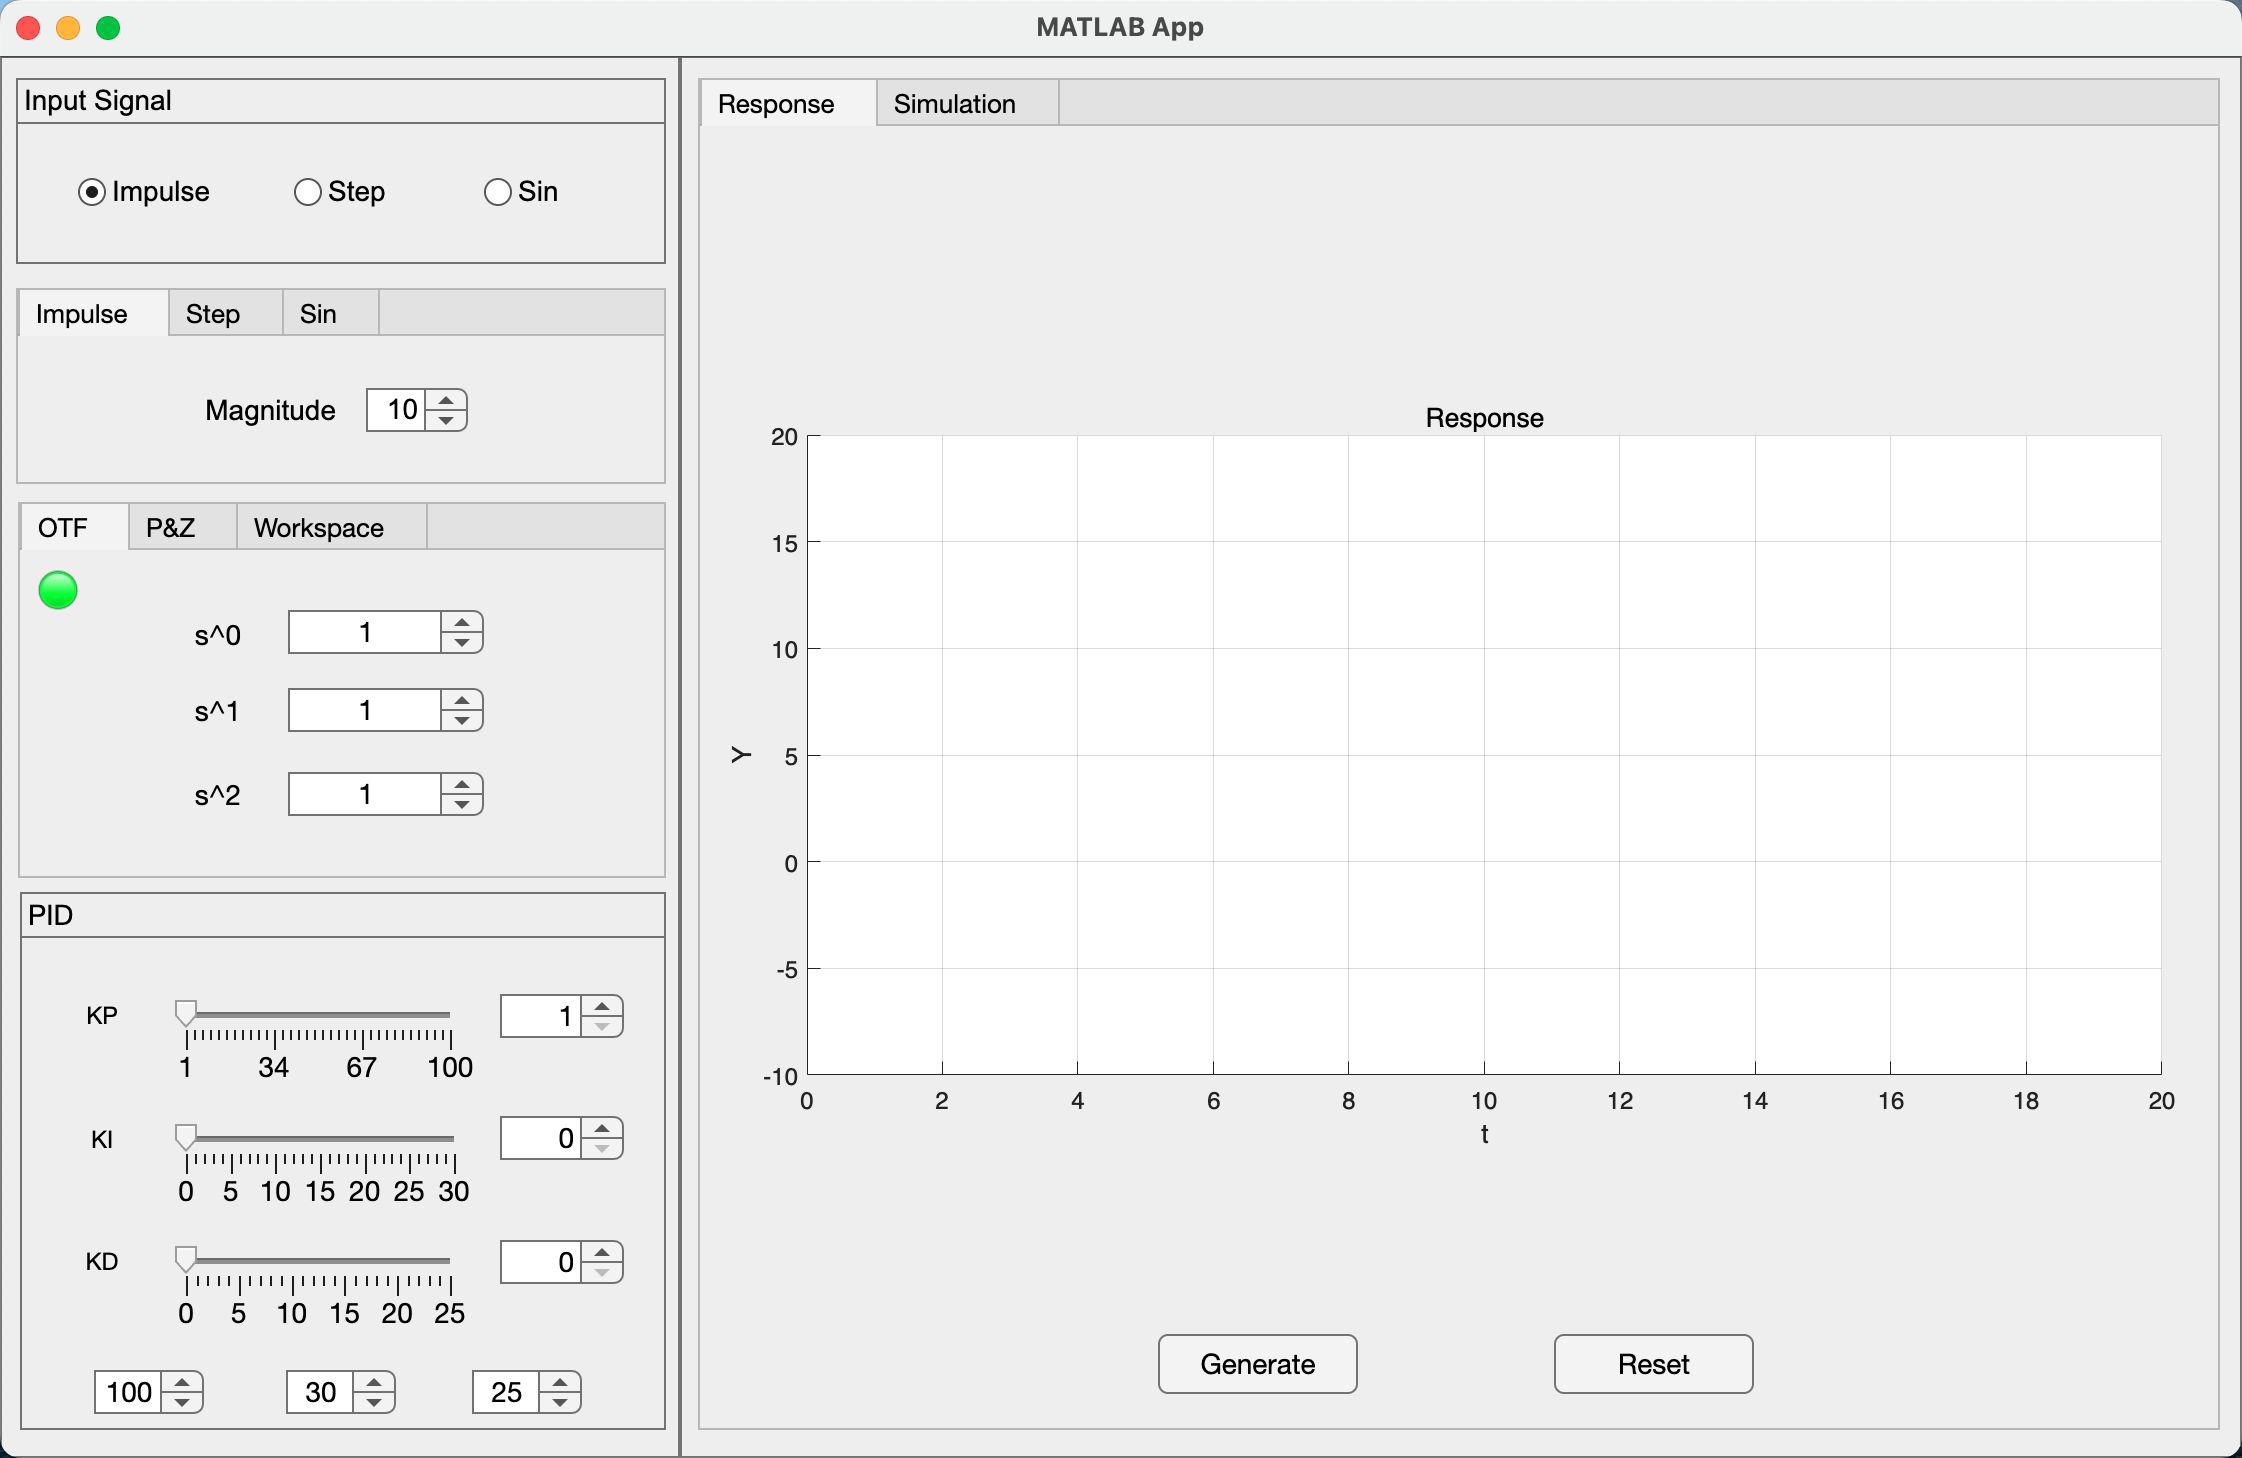
\includegraphics[width=\columnwidth]{Images/App.jpg}}
\caption{PID controller interface.}
\label{APP}
\end{figure}


\subsection{Input Signal Configuration}
The selection of the input signal includes options for impulse, step, and sinusoidal signals. A radio button group allows the user to select the desired signal type. The customization of input signal parameters is illustrated in Fig.\ref{fig:signal_config}, which provides options to customize the amplitude for step signals, both amplitude and delay for step signals, and amplitude and angular frequency for sinusoidal signals. Callback functions for the spinners ensure that modifying any parameter automatically updates the selected input signal.

\begin{figure}[!ht]
    \centering
    \begin{subfigure}[b]{0.5\textwidth}
        \centering
        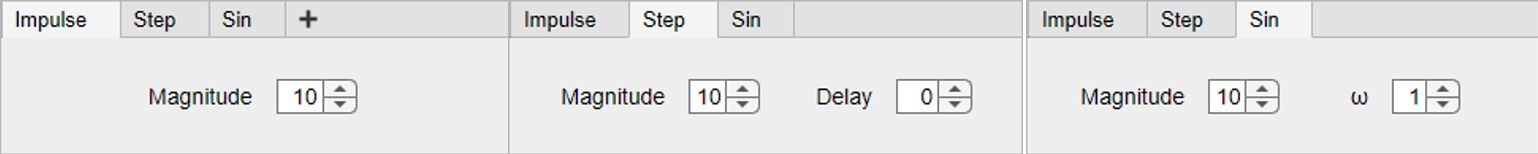
\includegraphics[width=\textwidth]{Images/Signal Config2.jpg}
        \caption{Signal configuration}
        \label{fig:signal_config}
    \end{subfigure}%
    \hfill % 添加一些水平空间
    \begin{subfigure}[b]{0.5\textwidth}
        \centering
        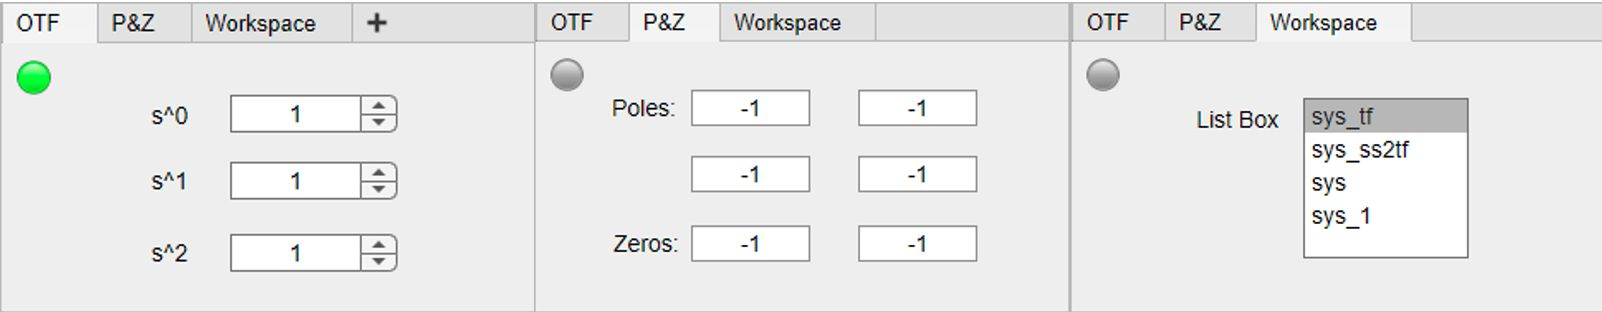
\includegraphics[width=\textwidth]{Images/TF Config.jpg}
        \caption{Transfer function configuration}
        \label{fig:tf_config}
    \end{subfigure}
    \caption{Comparison of signal and TF configurations}
    \label{fig:configs}
\end{figure}

\subsection{Transfer Function Configuration}
The definition of the transfer function for the controlled system is facilitated in three ways: open-loop transfer function (defining only the denominator of the transfer function), zeros and poles, and workspace import, as detailed in Fig.\ref{fig:configs}.

For the open-loop transfer function, coefficients for up to a second-order term can be modified via buttons. Zeros and poles configuration supports the input of up to four poles and two zeros via input fields, with constraints that inputs must be negative, ensuring that the transfer function remains stable with all zeros and poles on the left half of the complex plane.

Importing the transfer function from the workspace is crucial for practical PID control applications. By locating a transfer function with the same name in the workspace, we can integrate real-world transfer functions into the PID controller. Adjusting KP, KI, KD in conjunction with real-time response curves facilitates optimal tuning. Upon any parameter adjustment, a green light at the panel's top-left corner illuminates to indicate the selected method for defining the transfer function.

\subsection{Real-time PID Parameter Adjustment}

% \begin{figure}[!ht]
%     \centering
%     \begin{subfigure}[b]{0.5\textwidth}
%         \centering
%         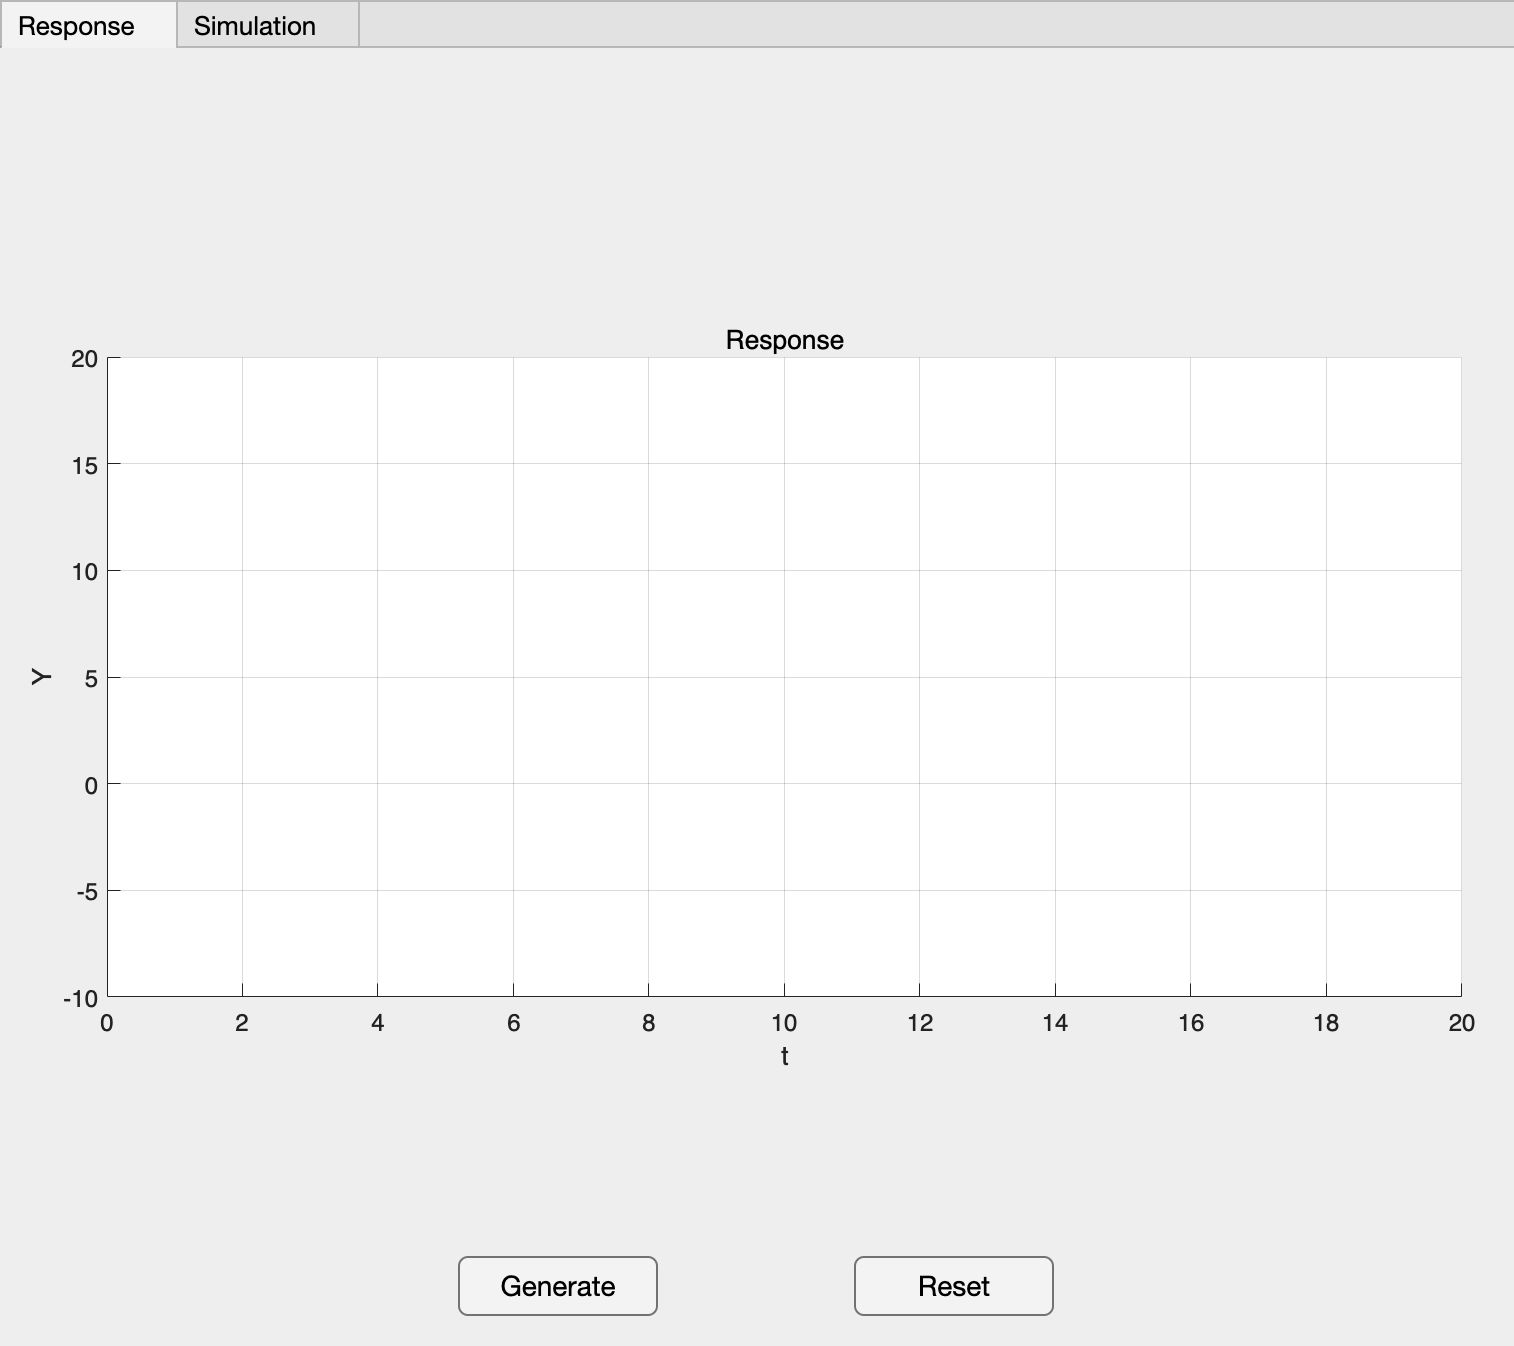
\includegraphics[width=\textwidth]{Images/Respond.jpg}
%         \caption{Response curve plotting window}
%         \label{fig:Respond}
%     \end{subfigure}%
%     \hfill % 添加一些水平空间
%     \begin{subfigure}[b]{0.5\textwidth}
%         \centering
%         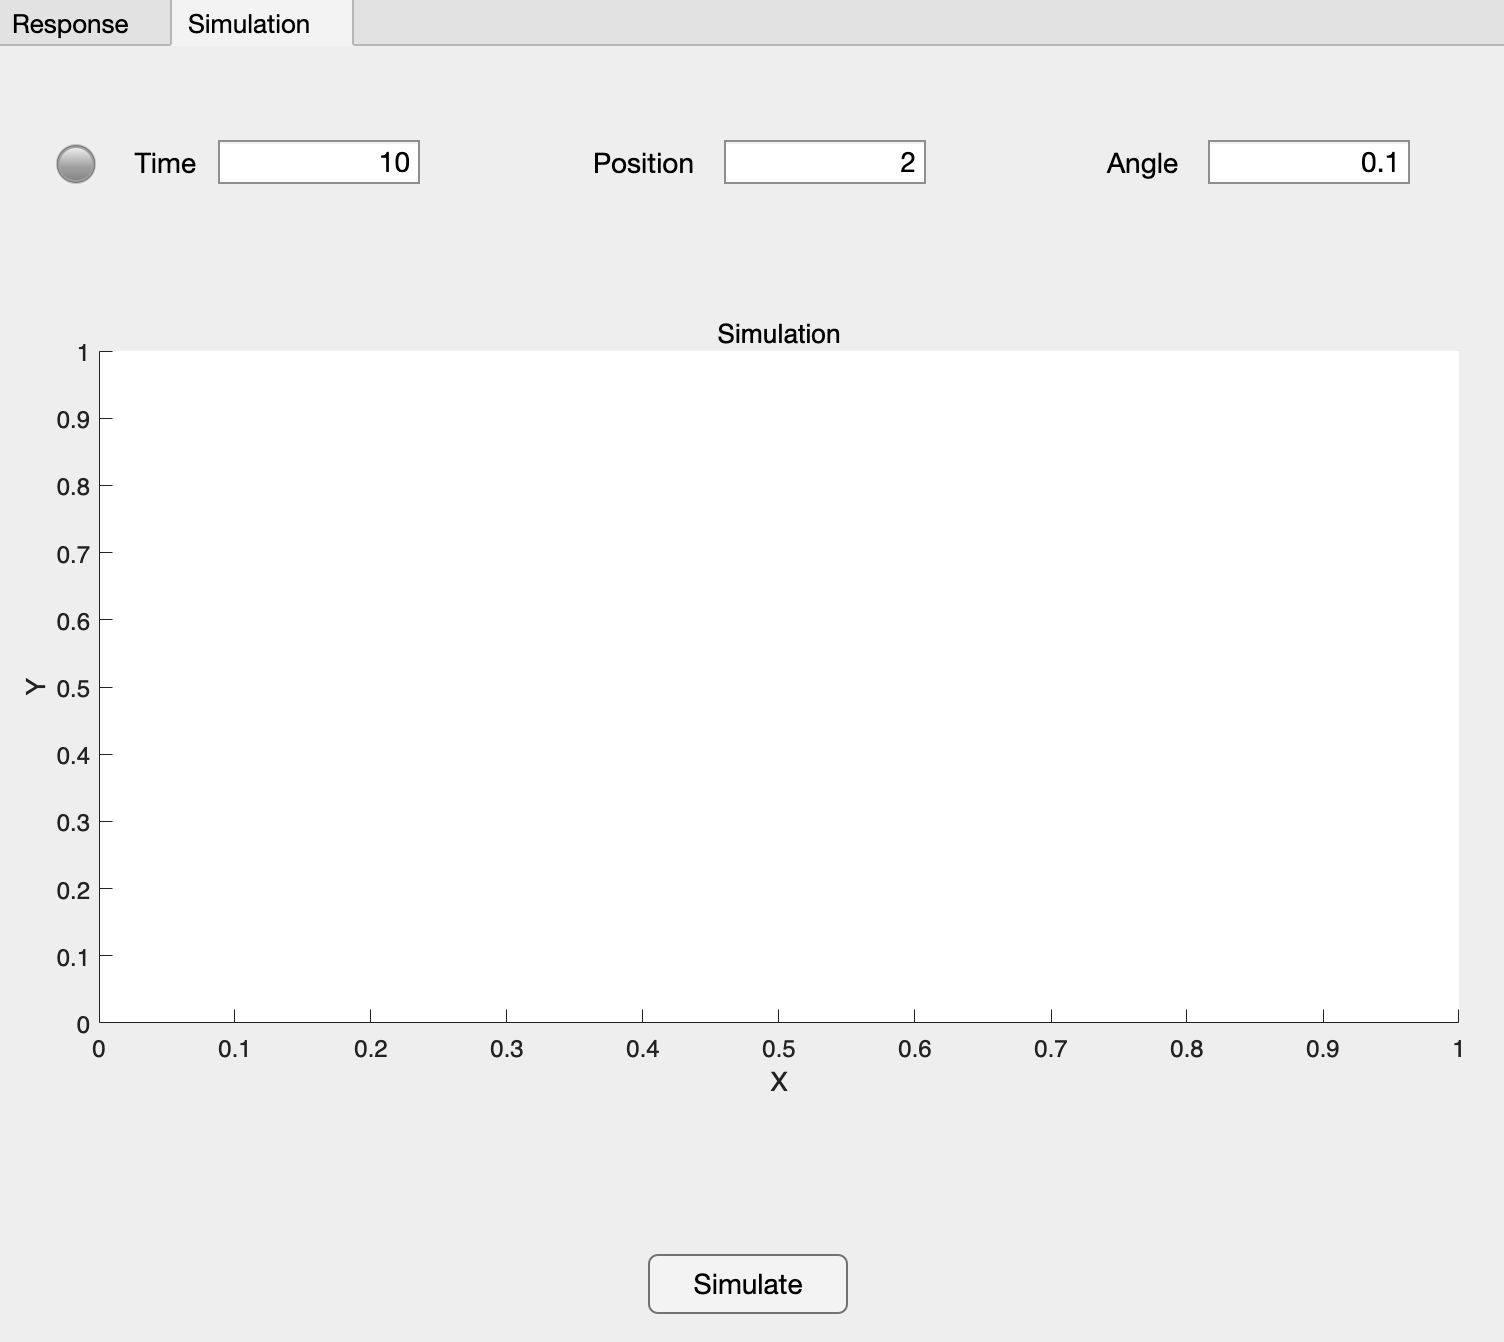
\includegraphics[width=\textwidth]{Images/sim.jpg}
%         \caption{Real-time simulation plotting window}
%         \label{fig:sim}
%     \end{subfigure}
%     \caption{Visualisation window preview image}
%     \label{fig:images_in_one_row}
% \end{figure}


The PID adjustment interface is located in the lower left part, and features three sliders corresponding to KP, KI, and KD. To display current slider values and allow for precise adjustments, there are spinners to the right of each slider. Changes in the slider's position automatically update the spinner displays, and vice versa. The three spinners at the bottom adjust the maximum values of the sliders to accommodate various scenarios requiring PID adjustments.

Following the adjustment of PID parameters, the effects on the controlled system’s transfer function are displayed in real-time, as illustrated in Fig.\ref{fig:nopid}. The interface below the response display includes two buttons, "Generate" and "Reset". Clicking "Generate" produces a new response curve upon changing the input signal or transfer function. Clicking "Reset" reverts all custom parameters to their default states and clears the response display.


\subsection{PID Simulation and Practical Applications}

\begin{figure}[!ht]
    \centering
    \begin{subfigure}[b]{0.5\textwidth}
        \centering
        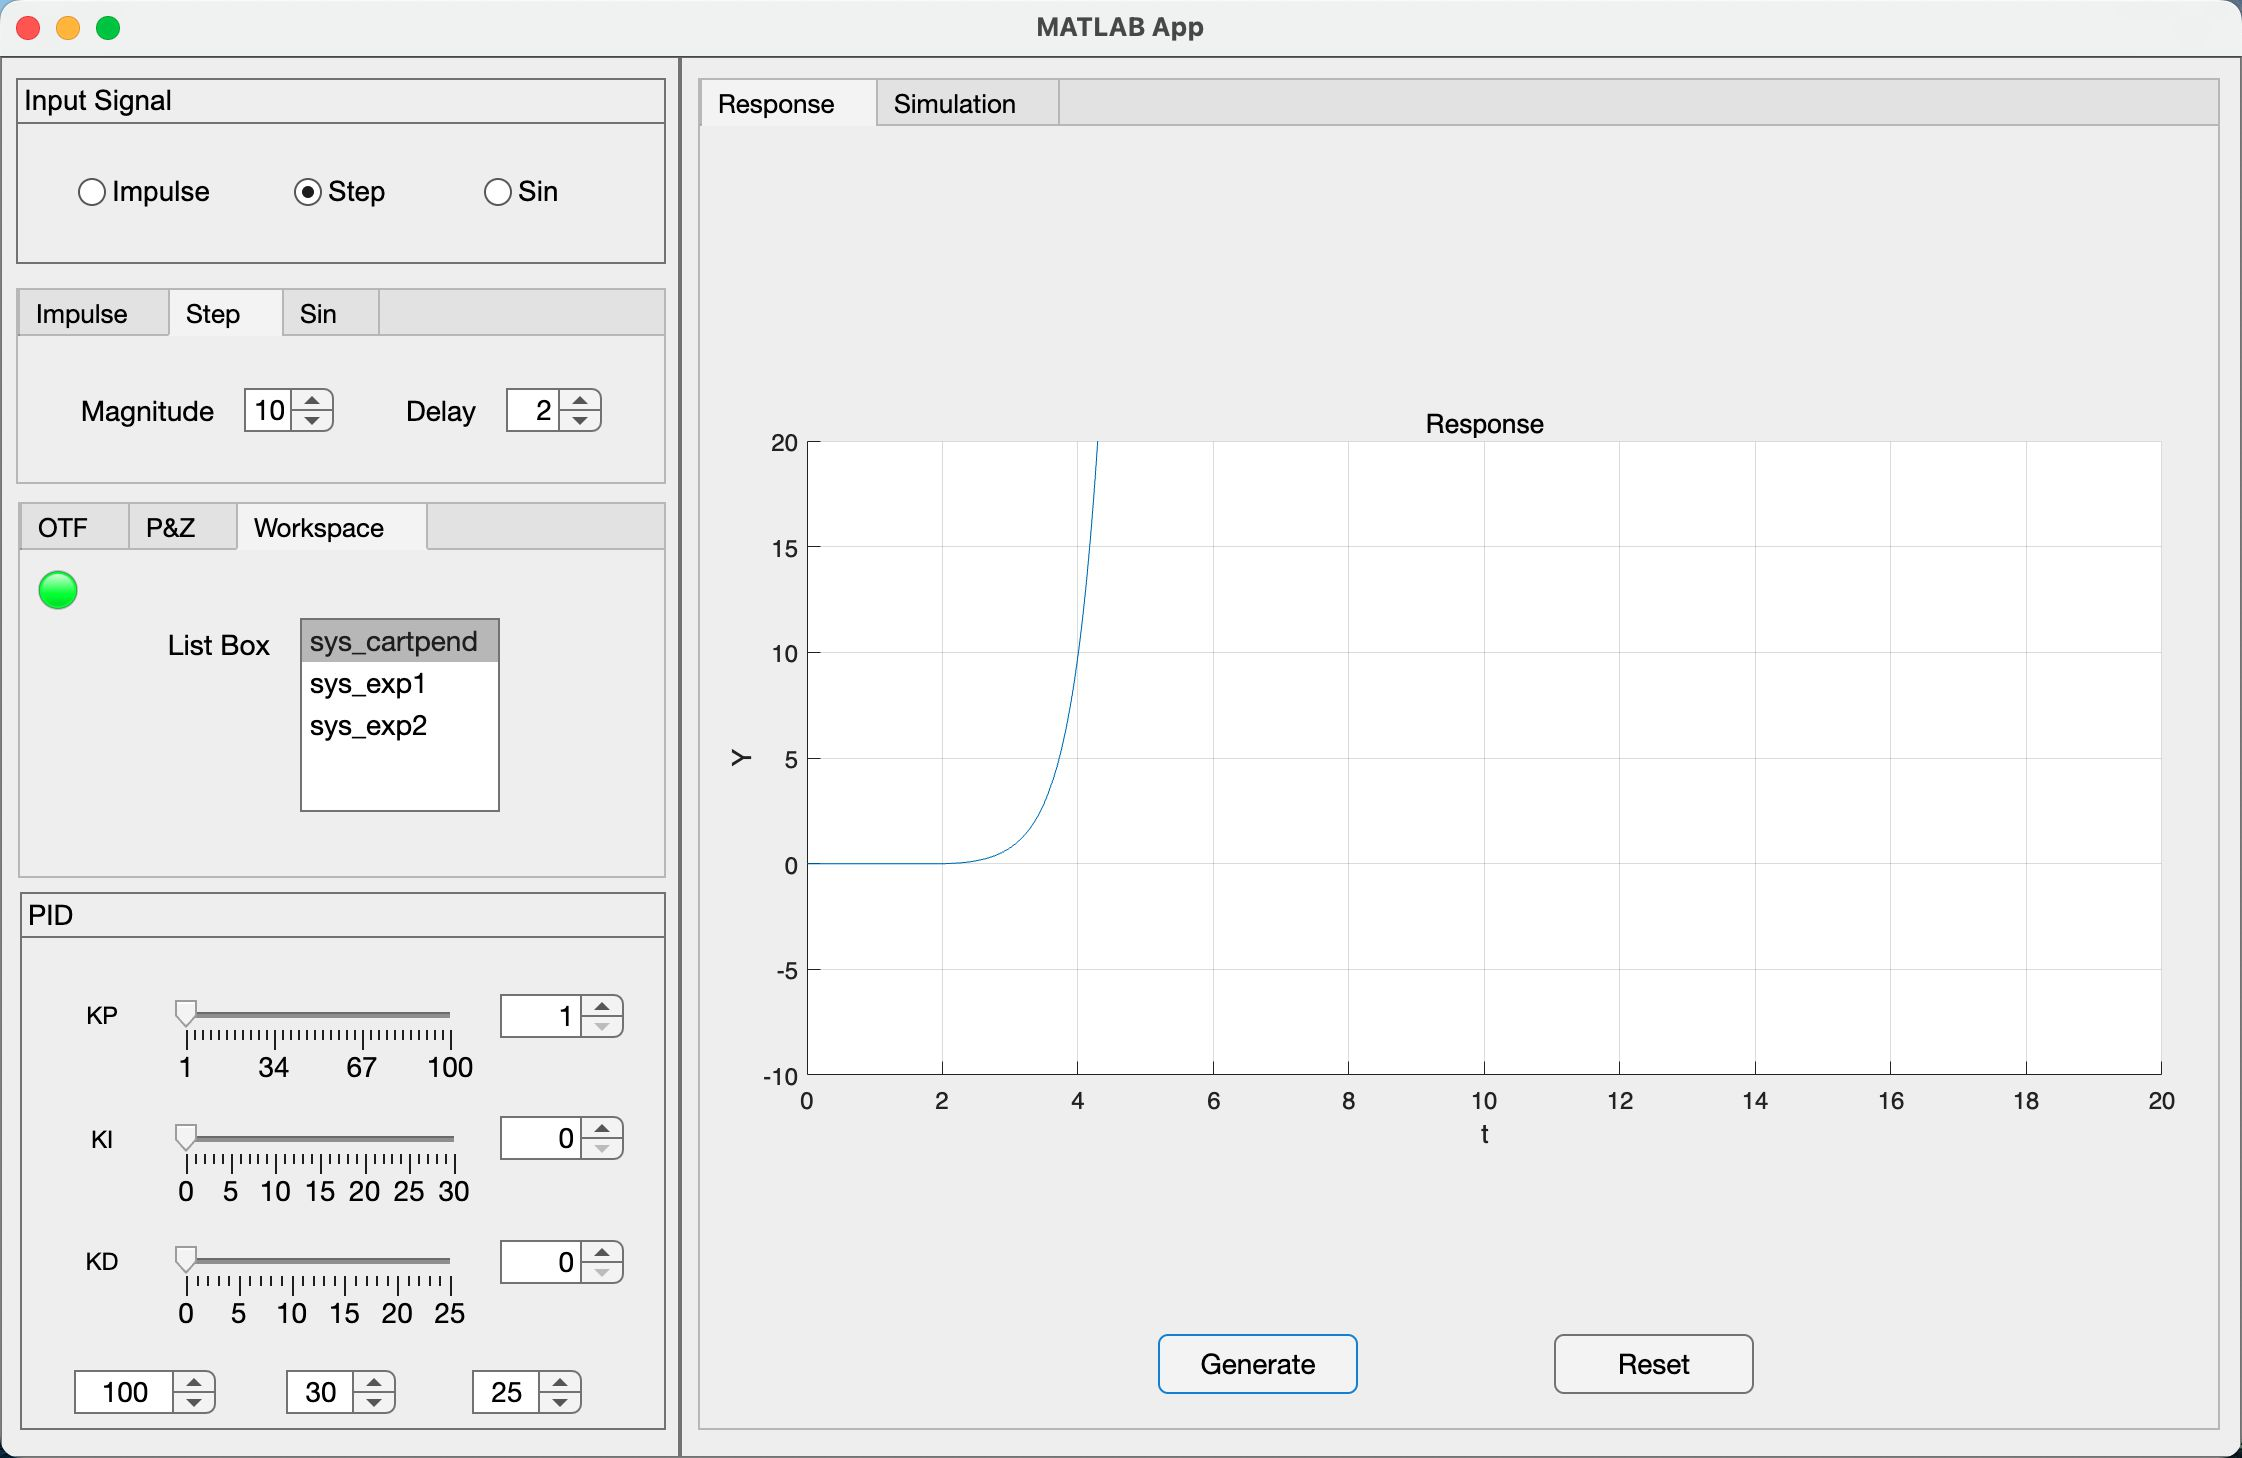
\includegraphics[width=\textwidth]{Images/nopid.jpg}
        \caption{Response curve without controller tuning}
        \label{fig:nopid}
    \end{subfigure}%
    \hfill % 添加一些水平空间
    \begin{subfigure}[b]{0.5\textwidth}
        \centering
        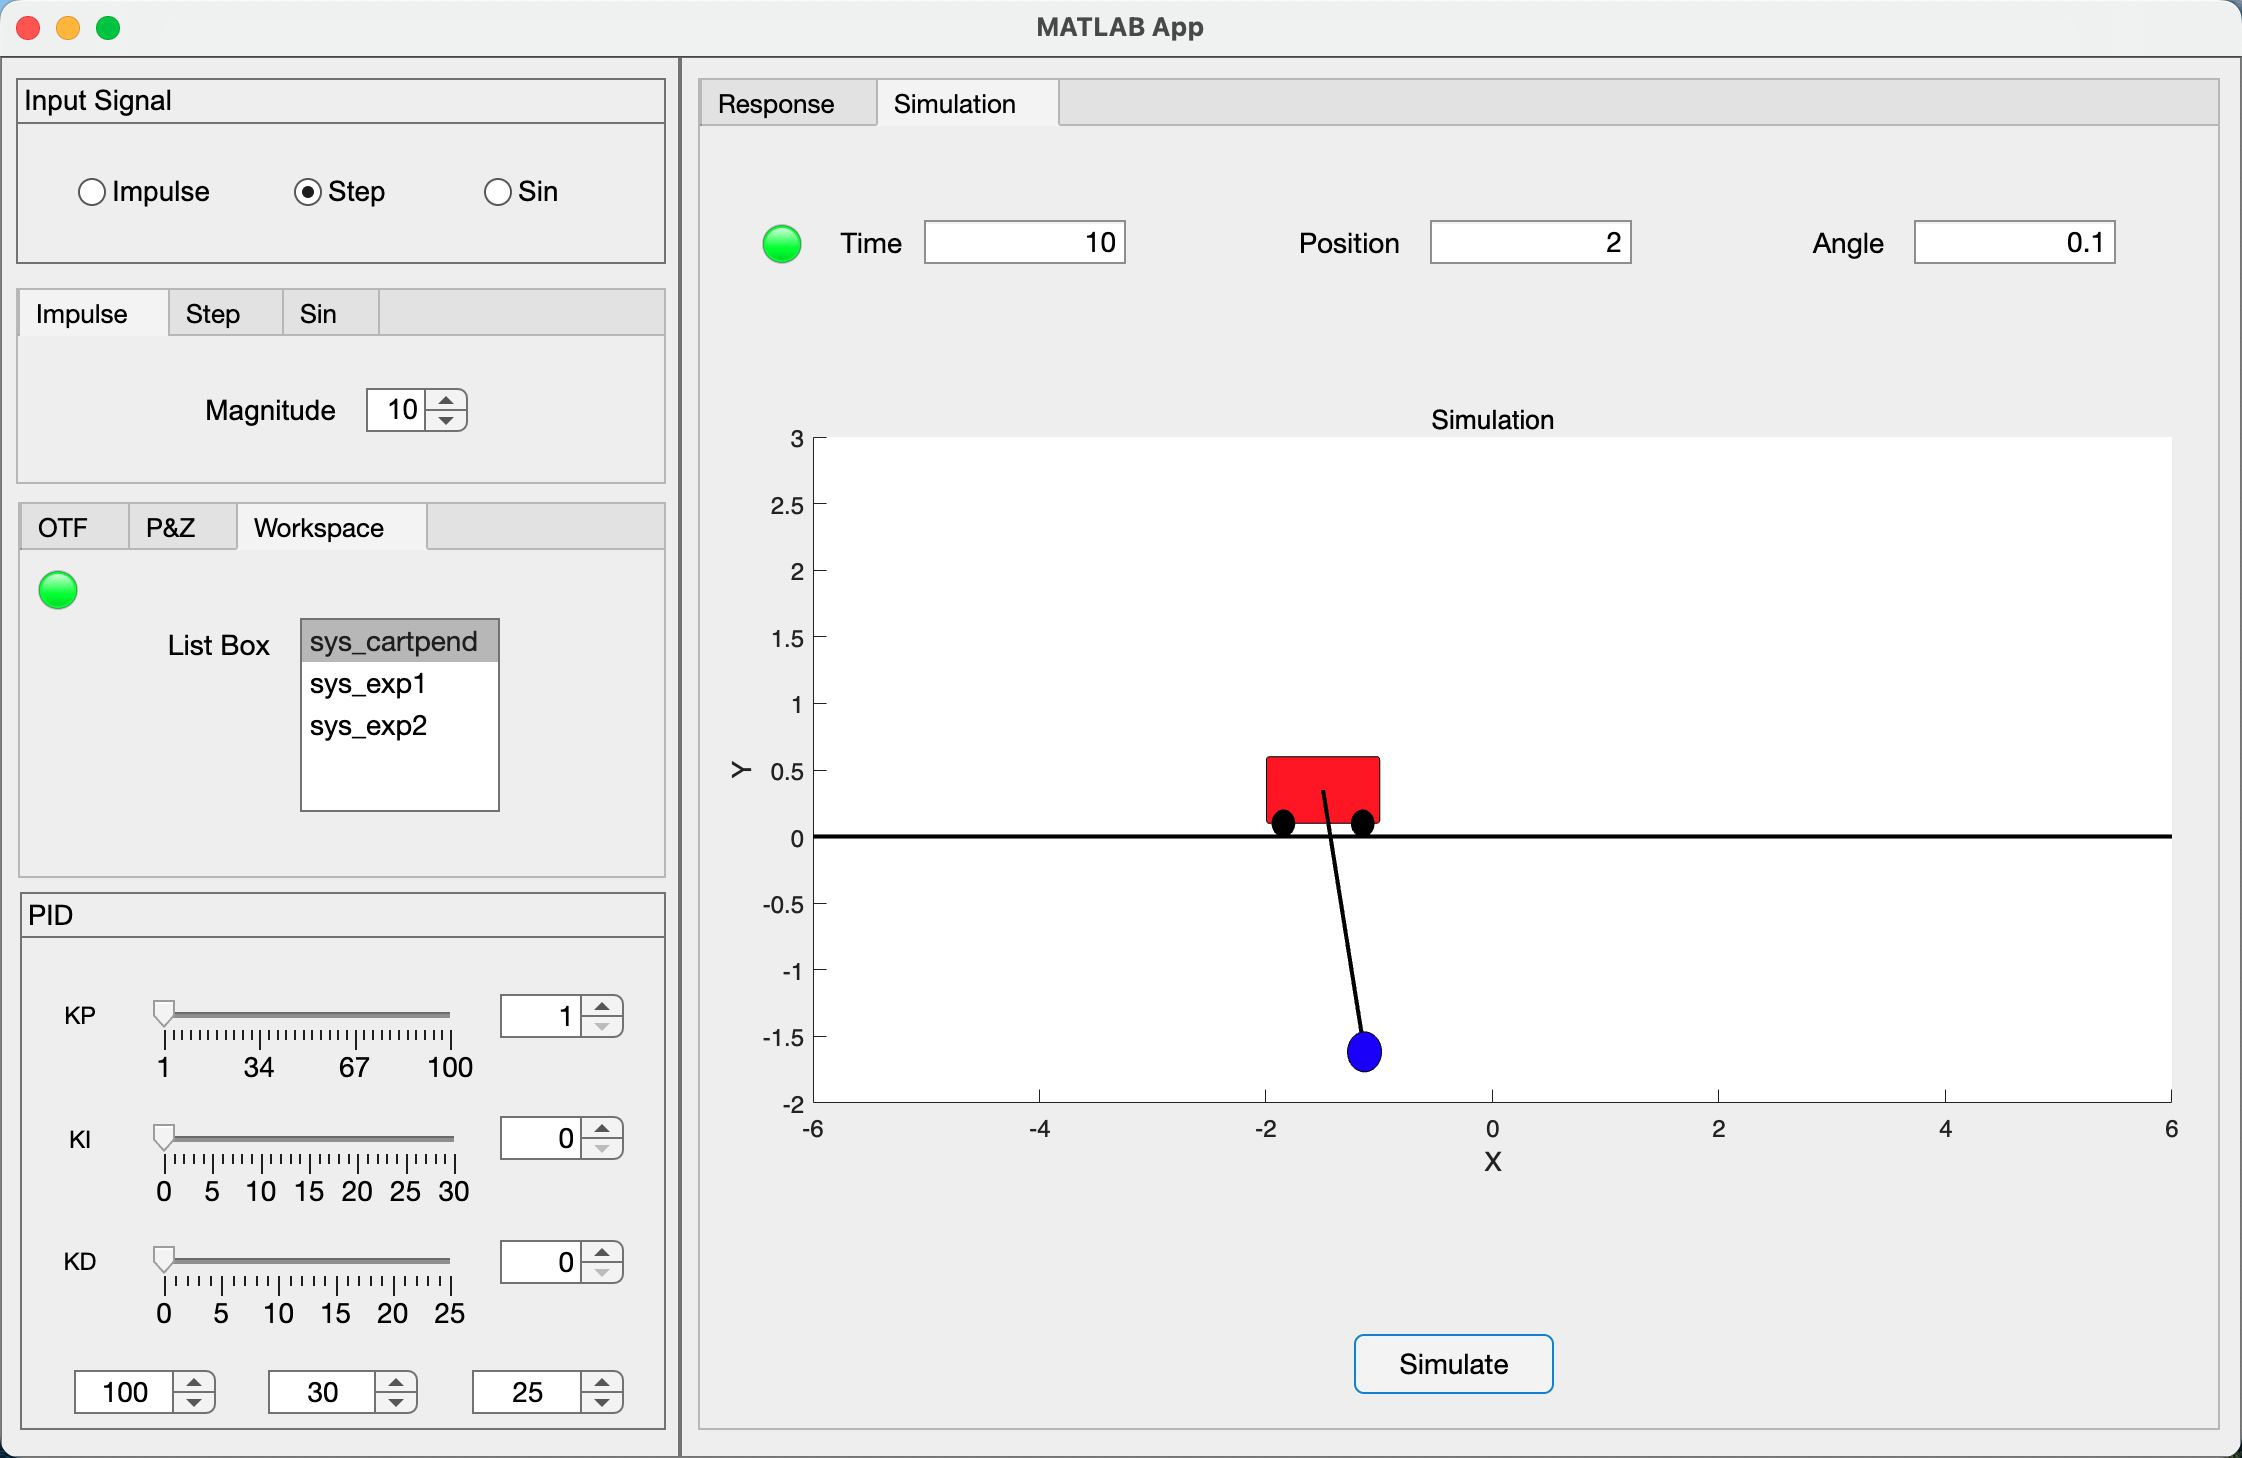
\includegraphics[width=\textwidth]{Images/Unsta.jpg}
        \caption{Visualisation without controller tuning}
        \label{fig:Unsta}
    \end{subfigure}
    \caption{Inverted pendulum system on cart without controller}
    \label{fig:side_by_side}
\end{figure}

\begin{figure}[!ht]
    \centering
    \begin{subfigure}[b]{0.5\textwidth}
        \centering
        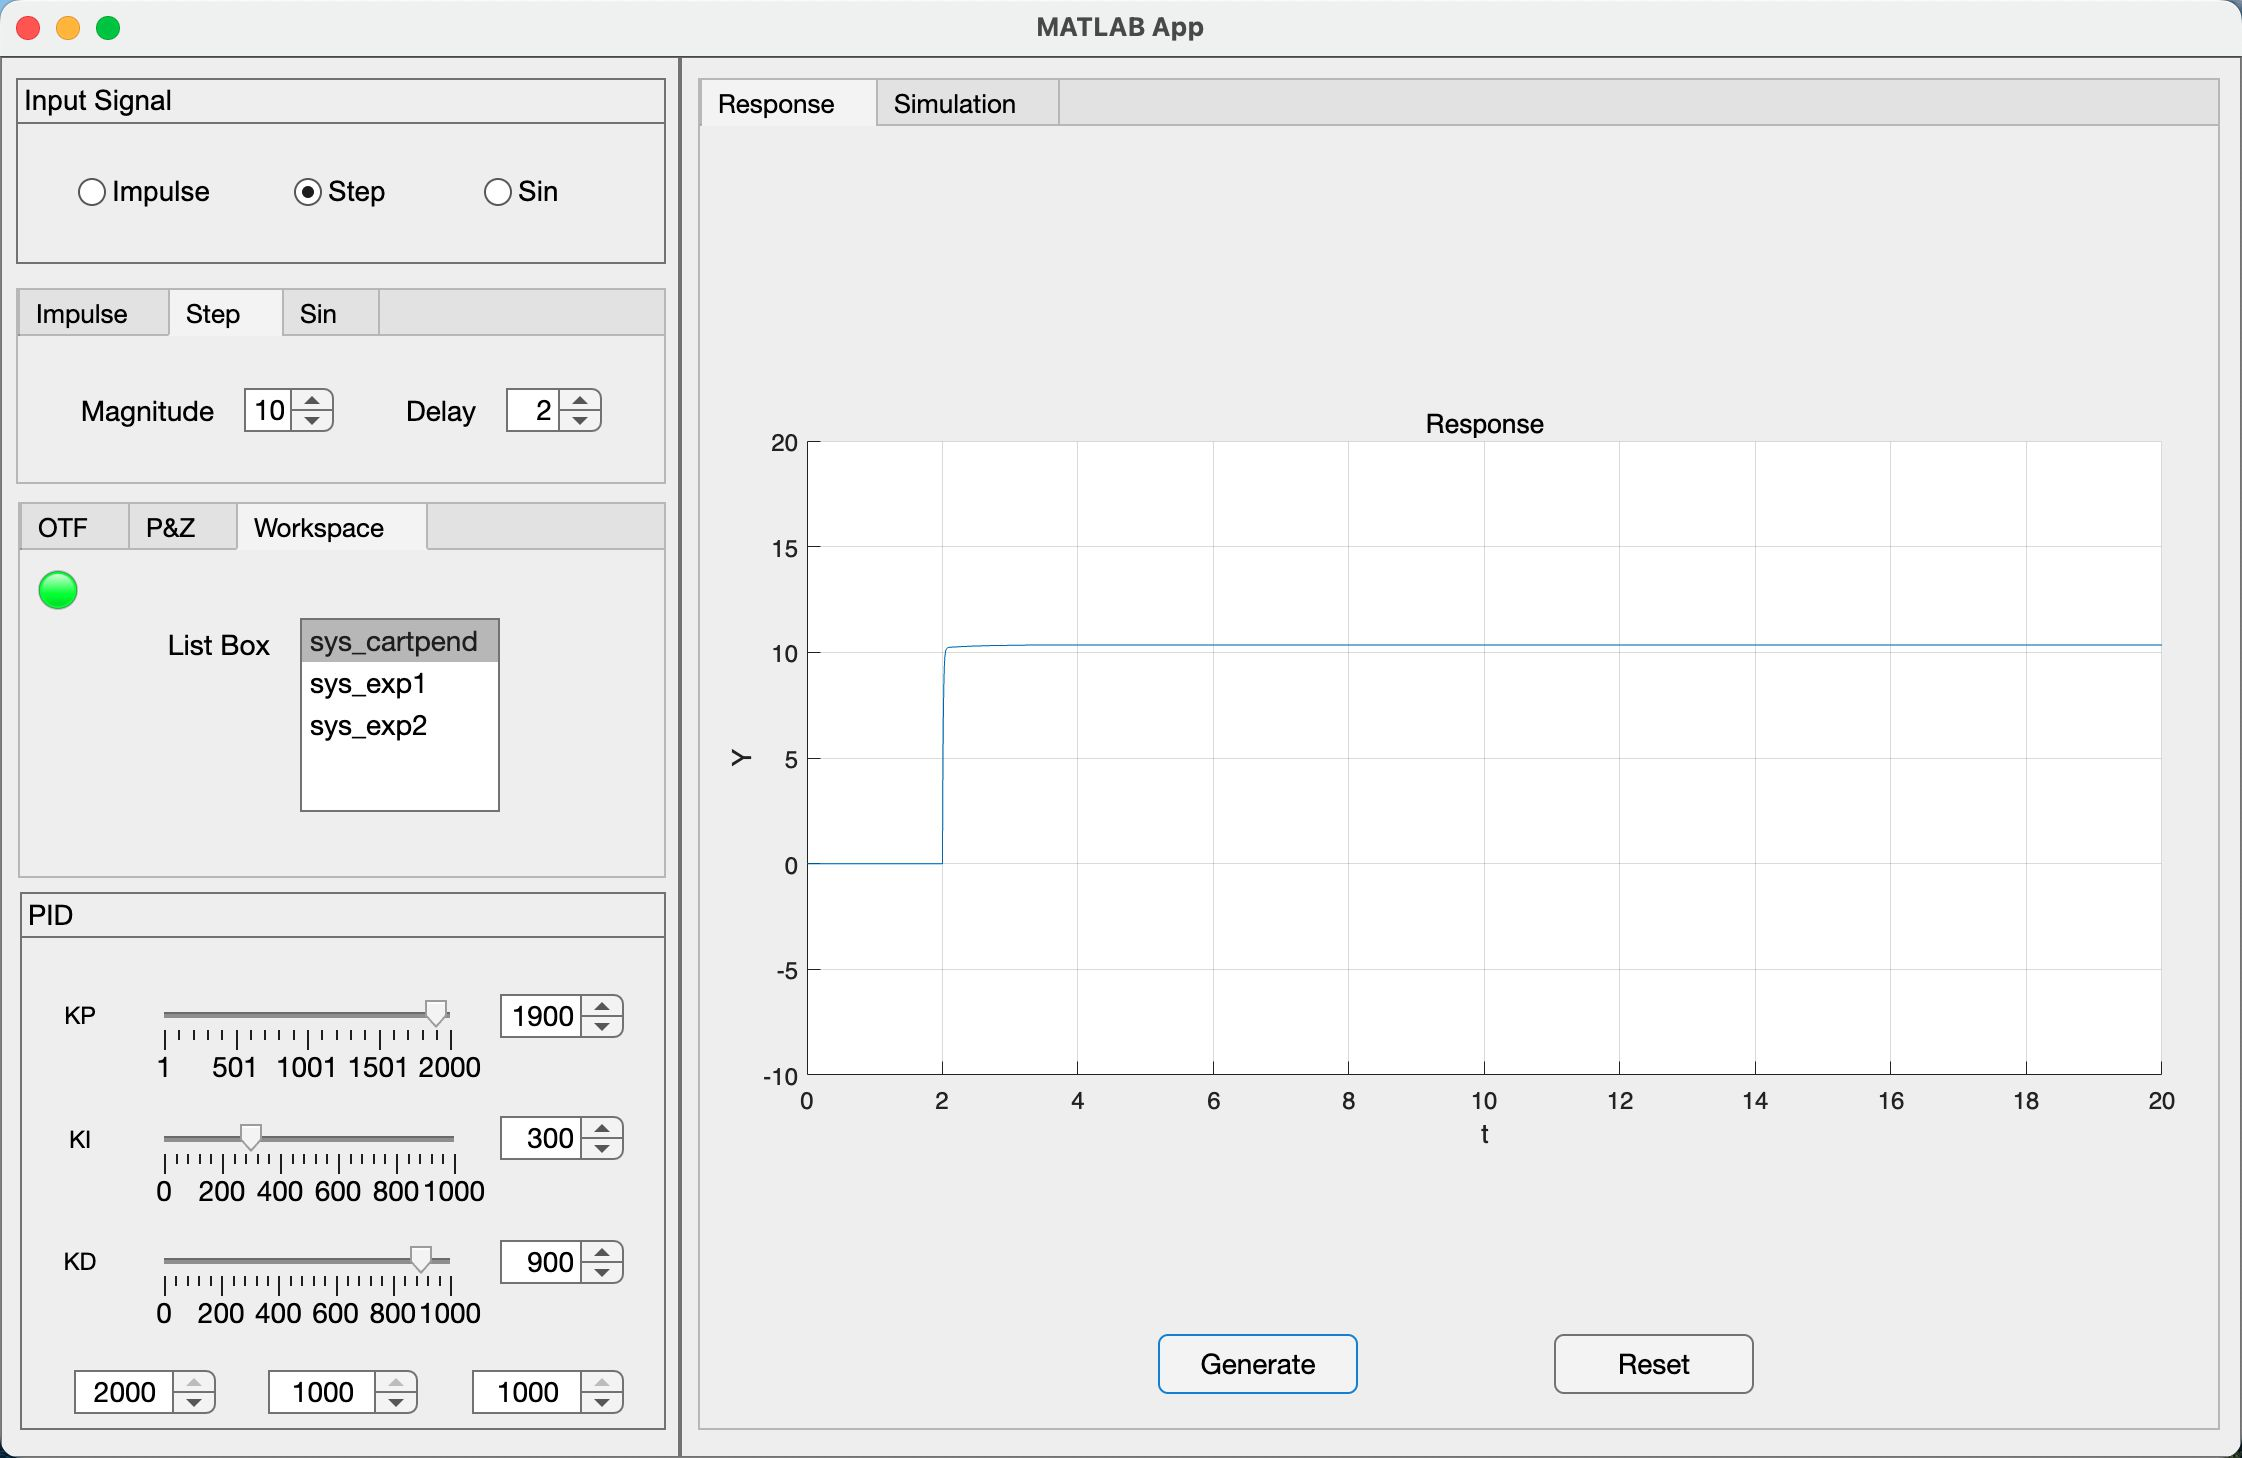
\includegraphics[width=\textwidth]{Images/PIDresult.jpg}
        \caption{Response curve with controller tuning}
        \label{fig:PIDresult}
    \end{subfigure}%
    \hfill % 添加一些水平空间
    \begin{subfigure}[b]{0.5\textwidth}
        \centering
        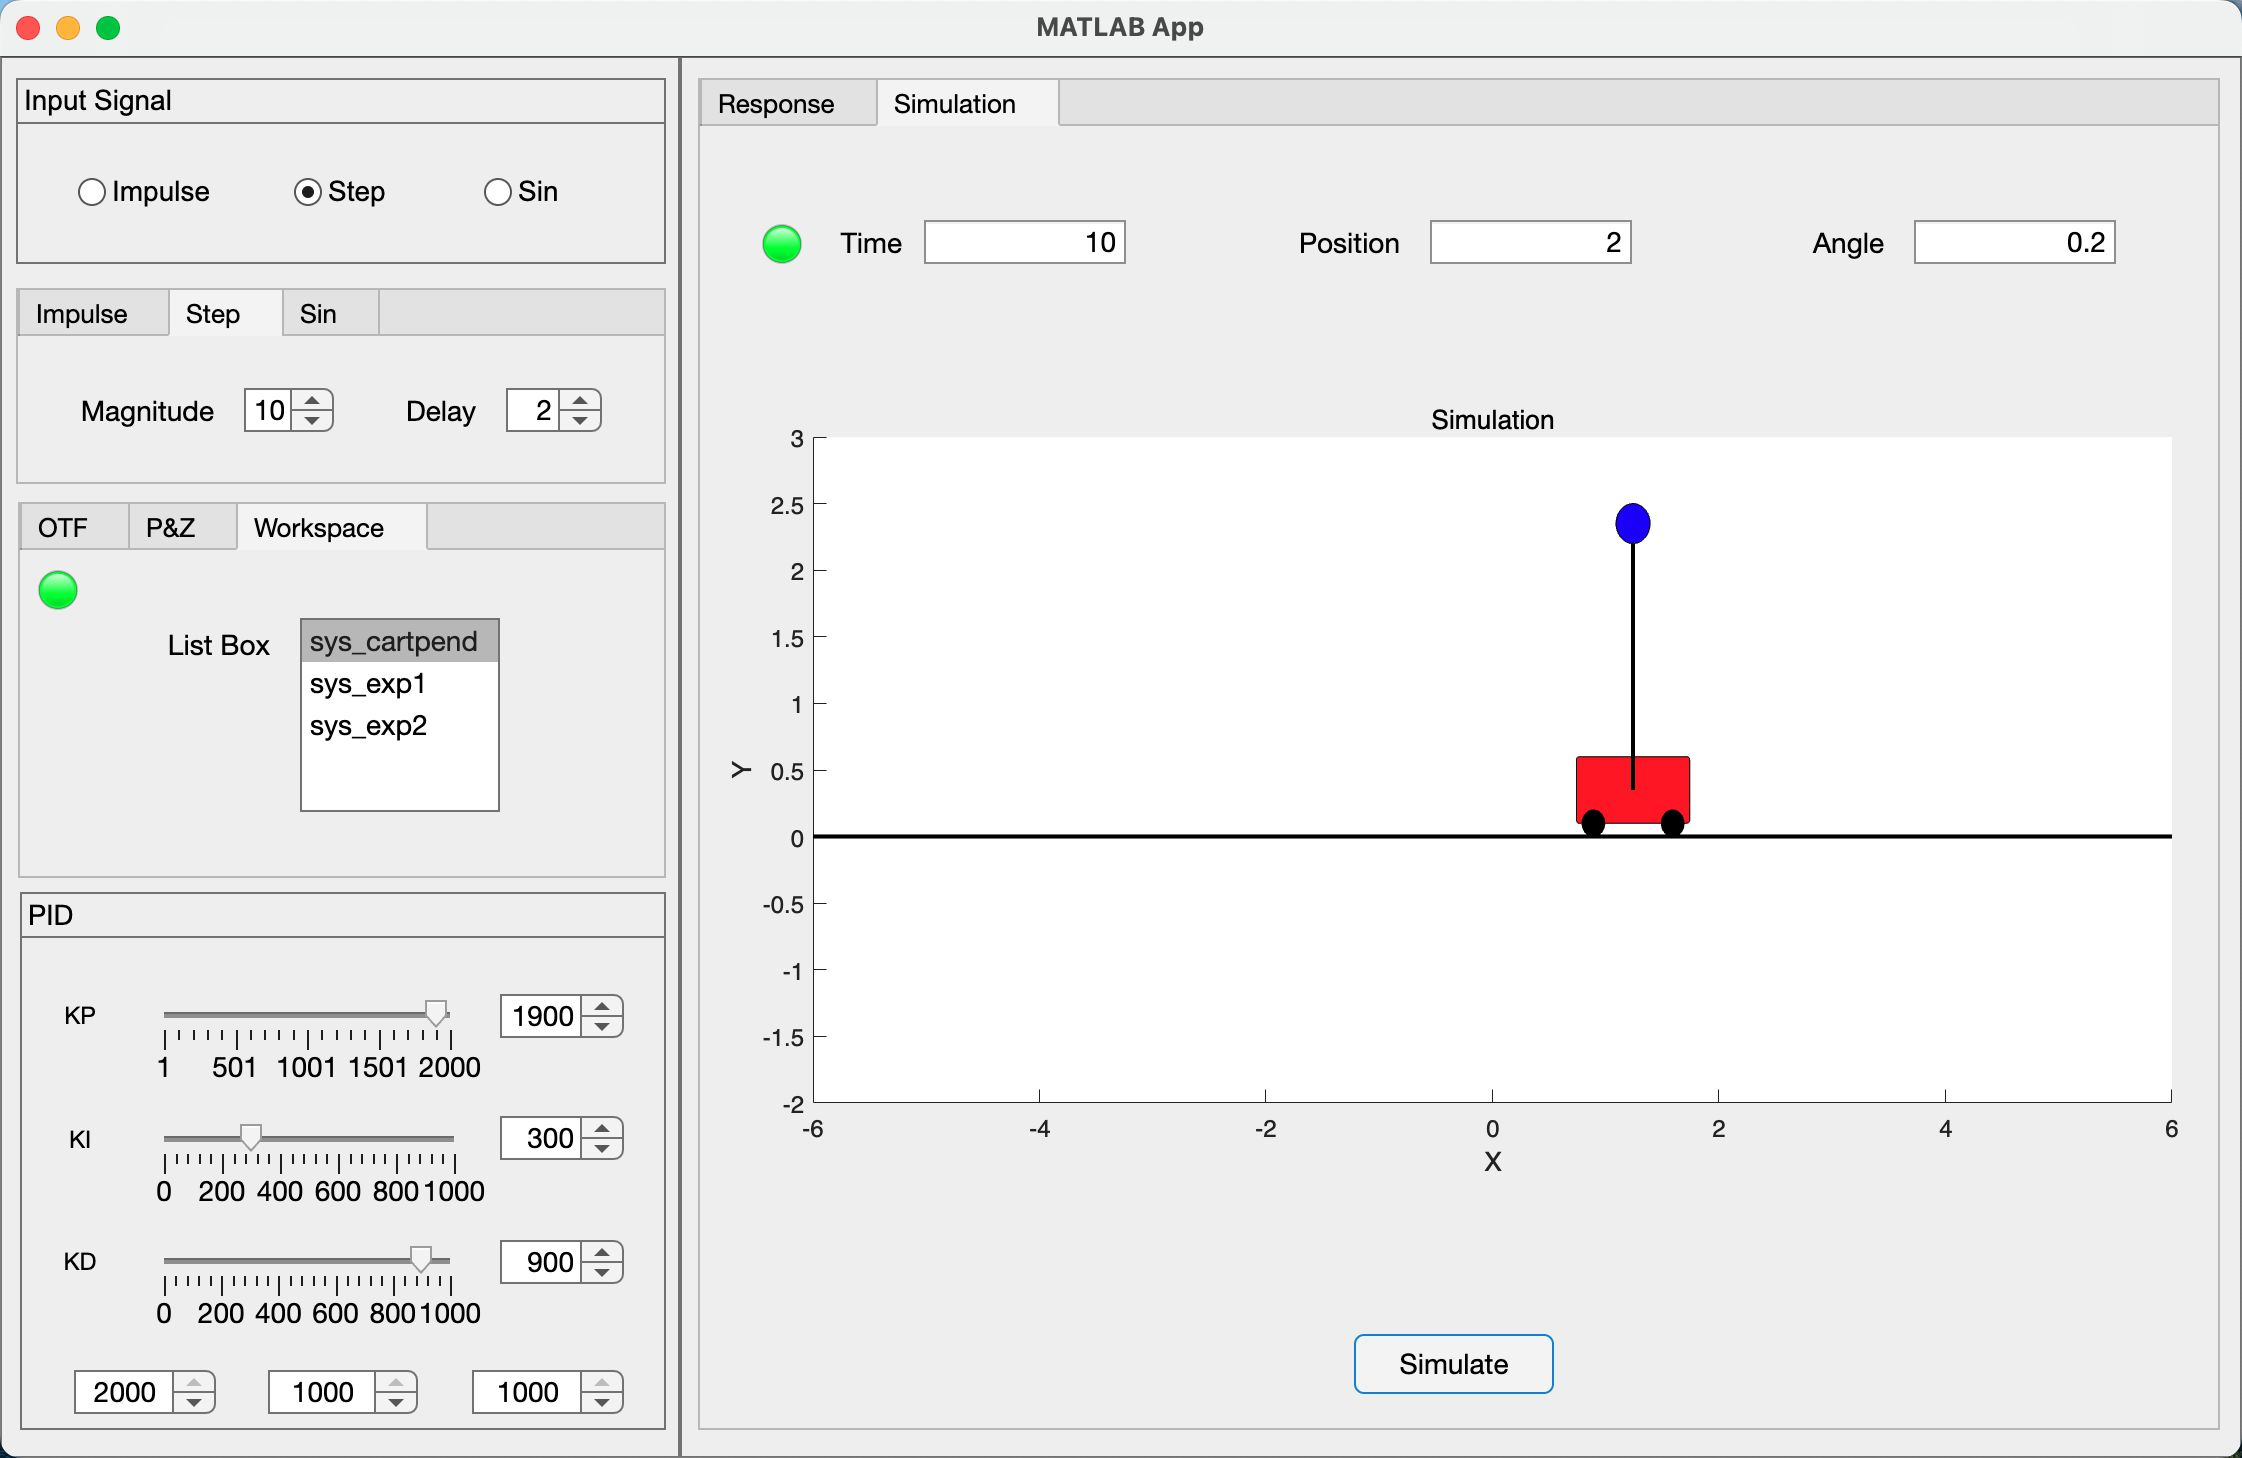
\includegraphics[width=\textwidth]{Images/PID siim.jpg}
        \caption{Visualisation with controller tuning}
        \label{fig:PIDsiim}
    \end{subfigure}
    \caption{Inverted pendulum system on cart with controller}
    \label{fig:123}
\end{figure}

The simulation panel offers three customizable parameters: simulation duration, initial position of the cart, and initial angle of the pendulum. Adjusting these parameters allows for various simulation outcomes. The "Simulate" button located at the bottom initiates the simulation process.

Importing the transfer function of the inverted pendulum from the workspace allows for simulation without PID control. The corresponding response curve and simulation results, shown in Fig.\ref{fig:Unsta}, indicate that the inverted pendulum cart is unstable without PID control, as evident from the response graph.

After adjusting the values of $K_p$,$K_i$and$K_d$, the corresponding simulation results can be observed. The following Fig.\ref{fig:123} shows the response curve and simulation effects when the system is stabilized.



\section{Conclusion}
The research detailed in this paper addresses the critical need for advanced control strategies in dynamic systems, specifically through the development of a sophisticated PID controller for an inverted pendulum on a cart. The controller's design integrates real-time simulation capabilities that significantly enhance the intuitiveness and effectiveness of PID tuning processes. The comprehensive development environment provided by MATLAB and APP Designer enabled the seamless integration of system modeling, control parameter adjustment, and visualization functionalities. Experimental validations confirm that the proposed PID controller not only stabilizes the inverted pendulum effectively but also offers robustness against disturbances and model uncertainties. This work not only advances the theoretical understanding and practical application of PID control in non-linear systems but also sets a foundation for future research on real-time control system optimization. Future work will focus on refining the controller's adaptive capabilities and expanding its application to other complex systems requiring precise and real-time feedback control.

\section*{Acknowledgment}

First and foremost, I would like to express my profound gratitude to the "Matlab Language and Simulation Practice" course and Assistant Professor Yue Ma. This course not only enabled me to master the use of MATLAB and Simulink but also deepened my understanding of their critical role in the field of control technology, particularly in the analysis of system responses and the design of controllers. The practical lessons taught me how to replicate the research content of papers and to master the standard format for writing academic papers in control studies, for which I am deeply thankful.

I also extend my thanks to my course partner. Together, we devoted substantial time and effort to completing this significant course project, often sacrificing sleep to ensure our report was of the highest quality. The support and companionship provided during crucial debugging processes were vital to the successful completion of our course report.

Additionally, I am grateful for the high-quality learning resources available online[9],[10],[11]. These resources, both easy to understand and creatively inspiring, greatly stimulated my ideas, especially in practical scenarios of controller design. I also appreciate the assistance of the GPT-4 large language model[12], which significantly enhanced my English expression skills, although there may still be some shortcomings in this process.

Lastly, I offer my sincere thanks to everyone who supported and helped me throughout this process. Your assistance was essential for the successful completion of this course report.

\section*{References}

\begin{thebibliography}{00}

\bibitem{bib1}Johnson M A, Moradi M H. PID control[M]. London, UK: Springer-Verlag London Limited, 2005.
\bibitem{bib2}Sushko A, Tedjarati A, Creus-Costa J, et al. Low cost, high endurance, altitude-controlled latex balloon for near-space research (ValBal)[C]//2017 IEEE Aerospace Conference. IEEE, 2017: 1-9.
\bibitem{bib3} Du H, Lv M, Li J, et al. Station-keeping performance analysis for high altitude balloon with altitude control system[J]. Aerospace Science and Technology, 2019, 92: 644-652.
\bibitem{bib4}Kafetzis I, Moysis L. Inverted Pendulum: A system with innumerable applications[J]. School of Mathematical Sciences, 2017.
\bibitem{bib5}Wang L. PID control system design and automatic tuning using MATLAB/Simulink[M]. John Wiley \&\ Sons, 2020.
\bibitem{bib6}Ang K H, Chong G, Li Y. PID control system analysis, design, and technology[J]. IEEE transactions on control systems technology, 2005, 13(4): 559-576.
\bibitem{bib7}Kumar P, Chakraborty K, Mukherjee R R, et al. Modelling and controller design of inverted pendulum[J]. International Journal of Advanced Research in Computer Engineering \&\ Technology (IJARCET), 2013, 2(1).
\bibitem{bib8}Brown P N, Byrne G D, Hindmarsh A C. VODE: A variable-coefficient ODE solver[J]. SIAM journal on scientific and statistical computing, 1989, 10(5): 1038-1051.
\bibitem{bib9}Tim. ACnD 4.Contorller Design[Online].Zhihu, 2022. Available: https://zhuanlan.zhihu.com/p/470029508
\bibitem{bib10}University of Michigan. Inverted Pendulum[Online].Website. Available: https://ctms.engin.umich.edu/CTMS/index.php
\bibitem{bib11}Steve B. Control Bootcamp[Online].Youtube, 2017. Available: https://www.youtube.com/@Eigensteve.
\bibitem{bib12}Jiao W, Wang W, Huang J, et al. Is ChatGPT a good translator? Yes with GPT-4 as the engine[J]. arXiv preprint arXiv:2301.08745, 2023.
\end{thebibliography}


\vspace{-80ex} % 调整这个值来减少空间
\begin{IEEEbiographynophoto}{Xiaotao Li(Leader),}
was responsible for setting the specific tasks and expected outcomes for the project titled "Design of a PID Controller with Practical Application Scenarios." His duties included conducting background research, gathering materials, and establishing the system model in MATLAB. He successfully implemented closed-loop PID control and visualization features, linking gain parameters with animations to achieve adjustable visual effects. In terms of writing the paper, Li was in charge of the overall structural arrangement and writing the sections in English. He also handled the integration of the final version of the manuscript, ensuring that all parts were cohesively presented.
\end{IEEEbiographynophoto}
\vspace{-90ex} % 调整这个值来减少空间
\begin{IEEEbiographynophoto}{Yikai Kang(Member),}
was tasked with developing the interface functionality of the PID controller using App design. He accomplished the integration of front-end and back-end interfaces, enabling the display of MATLAB results on the App interface. He organized and optimized the code to ensure the functionality of all features. In the writing phase of the paper, Kang was responsible for demonstrating the results and proofreading the format and content of the manuscript to maintain high standards in presentation and accuracy.
\end{IEEEbiographynophoto}



\end{document}
